\documentclass[notitlepage]{article}
\usepackage{amsmath, amssymb}
\usepackage{enumerate}
\usepackage[margin=1in]{geometry}
\usepackage{tikz}
\usepackage{standalone}
\usepackage{graphicx}
\usepackage{subfig}
\usepackage{cases}
\usepackage{xcolor}
\DeclareMathOperator{\Var}{Var}
\DeclareMathOperator{\Cov}{Cov}
\DeclareMathOperator{\Corr}{Corr}
\DeclareMathOperator{\ACF}{ACF}
\DeclareMathOperator{\PACF}{PACF}

\setlength\parindent{0pt}

\begin{document}

Author: Jacky Leung

These notes are for ECON 4304: Time Series Econometrics and Business Forecasting at HKUST. The primary focus is on the mathematical derivation and analysis of time series models, and empirical applications are left for independent study. The content is adapted from Dr. Eric Ng's course materials, with the main differences being minor adjustments to the content sequence and a greater emphasis on matrix algebra.

\section{Modeling Time Series Data: ARMA Models}

\subsection{Introduction}

\begin{itemize}
    \item What is a time series?
    \begin{itemize}
        \item A natural ordering by dates: $1, 2, \dots, t, t+1, \dots, T$.
        \item A time series is a sequence of observations ordered by dates: \(\{y_1, y_2, \dots, y_t, y_{t+1}, \dots, y_T\}\).
    \end{itemize}
    \item Motivation of time series analysis and modeling:
    \begin{itemize}
        \item Understanding past data, forecasting future data.
    \end{itemize}
    \item Some features in real-life time series:
    \begin{itemize}
        \item Trend, Seasonality, Cyclicality, and Irregularity.
        \item Current shock \(u_t\) tends to affect both present variable \(y_t\) and future variables \(y_{t+1}, y_{t+2}, \dots\).
        \item Structural breaks (sudden changes over time) in mean, variance, and/or regression coefficients.
        \item Spurious regression: Strong relationship between completely unrelated time series variables.
        \item Autocorrelated: The present observation is correlated with both past and future observations:
        \[
        \Cov(y_{t-1}, y_t) \ne 0, \; \Cov(y_t, y_{t+1}) \ne 0
        \]
    \end{itemize}
\end{itemize}

\subsection{Stationarity}

\begin{itemize}
    \item Our models and forecasting primarily focus on \textbf{covariance stationary}, or simply \textbf{stationary} time series data, which has the following properties:
    \begin{align*}
        \mathbb{E}[y_t] &=\mu < \infty \\
        \mathbb{E}[(y_t-\mu)^2] &= \Var(y_t) < \infty \\
        \mathbb{E}[(y_t-\mu)(y_{t+j}-\mu)] &= \Cov(y_t, y_{t+j}) = \gamma_j < \infty \text{ for all } j = 0, 1, 2, \dots
    \end{align*}
    \item \(\gamma_j\) is called \textbf{autocovariance}. Note that \(\gamma_0 = \Var(y_t)\).
    \item Mean, variance, and autocovariance do not change over time for a stationary process.
    \item For a stationary process, \(\Cov(y_{t-j}, y_t) = \Cov(y_t, y_{t+j}) = \gamma_j\).
    \item Some examples of stationary/nonstationary processes:
    \begin{itemize}
        \item A growing trend is not stationary as the mean is increasing over time.
        
        \begin{center}
            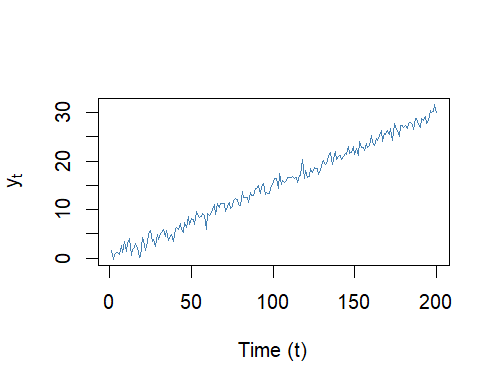
\includegraphics[width=0.5\linewidth, trim={0 0.5cm 0 1.5cm},clip]{growing.png}
        \end{center}
        
        \item \textbf{White noise process}:
        \[
        y_t = u_t
        \]
        where \(\mathbb{E}[u_t]=0, \Var(u_t)=\gamma_0=\sigma^2\) and \(\gamma_j = 0\) by definition, which is stationary. Oftentimes we take \(u_t \overset{\text{i.i.d.}}{\sim} \mathcal{N}(0,\sigma^2)\).

        \begin{center}
            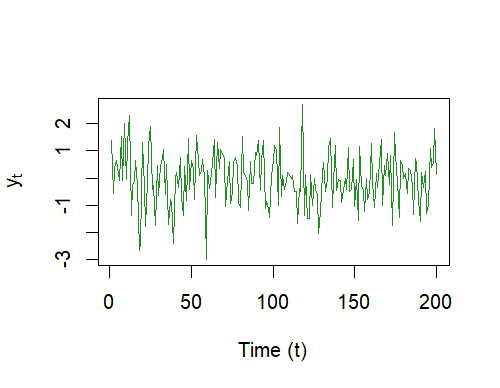
\includegraphics[width=0.5\linewidth, trim={0 0.5cm 0 1.5cm},clip]{whitenoise.png}
        \end{center}
        
        \item \textbf{Random walk process} (without drift):
        \[
        y_t = y_{t-1} + u_t
        \]
        is not stationary, because:
        \[
            \Var(y_t) = \Var(y_0 + \sum_{i=1}^t u_i)
            = \Var(\sum_{i=1}^t u_i)
            = \sum_{i=1}^t \Var(u_i)
            = t\sigma^2
        \]

        \begin{center}
            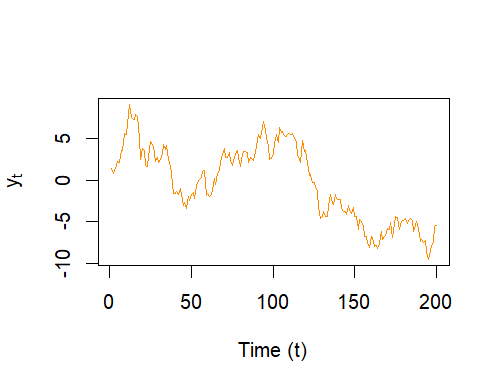
\includegraphics[width=0.5\linewidth, trim={0 0.5cm 0 1.5cm},clip]{randomwalk.png}
        \end{center}
        
        \item A time series with \textbf{structural break} is not stationary:
        \[
        y_t =
        \begin{cases}
            \mu_1 + u_t &\text{if } t<T_0\\
            \mu_2+ u_t &\text{if } t\ge T_0
        \end{cases}
        \]

        \begin{center}
            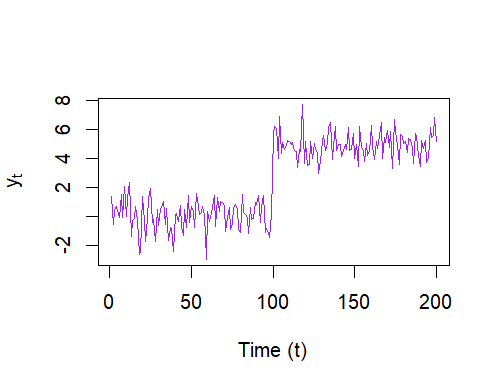
\includegraphics[width=0.5\linewidth, trim={0 0.5cm 0 1.5cm},clip]{break.png}
        \end{center}
    \end{itemize}
\end{itemize}

\subsection{AR model, ACF and PACF}

\begin{itemize}
    \item An \textbf{autoregressive model} with order \(p\), AR(\(p\)), is defined as:
    \[
    y_t = c + \sum_{j=1}^p \phi_j y_{t-j} + u_t = c + \phi_1 y_{t-1} + \dots + \phi_p y_{t-p}  + u_t
    \]
    where \(u_t\) is a white noise process.
    \item In practice, one of the most widely used model is AR(1):
    \[
    y_t = c + \phi y_{t-1} + u_t
    \]
    \item For an AR(1) to be stationary, we must have \(|\phi| < 1\), because:
    \[
    \Var(y_t) = \Var(c + \phi y_{t-1} + u_t) = \phi^2\Var(y_{t-1}) + \sigma^2
    \]
    For a stationary model, \(\Var(y_t) = \Var(y_{t-1}) = \gamma_0\), thus:
    \[
    \Var(y_t) = \gamma_0 = \frac{\sigma^2}{1-\phi^2}
    \]
    Hence, \(\Var(y_t) > 0\) only if \(|\phi| < 1\).
    \item For an AR(\(p\)) to be stationary, all roots for the characteristic equation \(z^p - \sum_{j=1}^p \phi_j z^{p-j}=0\) must lie within a complex unit circle.
    
    \item Apart from the mean, variance and autocovariance of a time series, we are also naturally interested in the \textbf{autocorrelation}:
    \[
    \rho_j = \frac{\Cov(y_{t-j}, y_t)}{\Var(y_t)}
    \]
    \item Computing \(\rho_j\) for all \(j\), we can obtain the \textbf{autocorrelation function}, ACF(\(j\)).
    \item For example, for an AR(1): \(y_t = c + \phi y_{t-1} + u_t\),
    \begin{align*}
        \gamma_1 &= \Cov(y_t, y_{t-1}) = \Cov(c + \phi y_{t-1} + u_t, y_{t-1}) = \phi \gamma_0 \\
        \gamma_2 &= \Cov(y_t, y_{t-2}) = \Cov(c + \phi y_{t-1} + u_t, y_{t-2}) = \phi \gamma_1 = \phi^2\gamma_0
    \end{align*}
    Thus, we can deduce that:
    \[
    \gamma_j = \phi^j \gamma_0
    \]
    It follows that:
    \[
    \rho_j = \frac{\gamma_j}{\gamma_0} = \phi^j
    \]
    \item For AR models with higher order, this method isn't as useful since different \(y_{t-j}\) terms are correlated.
    \item Instead, we can derive something called \textbf{Yule-Walker equations}. For simplicity, consider an AR(2) with zero mean: \(y_t = \phi_1 y_{t-1} + \phi_2 y_{t-2} + u_t\), then we can make use of a property:
    \[
    \gamma_j = \mathbb{E}[(y_t-\mu)(y_{t-j}-\mu)] = \mathbb{E}[y_ty_{t-j}]
    \]
    We can derive that:
    \begin{align*}
        y_ty_{t-j} &= \phi_1 y_{t-1}y_{t-j} + \phi_2 y_{t-2}y_{t-j} + u_ty_{t-j} \\
        \mathbb{E}[y_ty_{t-j}] &= \phi_1 \mathbb{E}[y_{t-1}y_{t-j}] + \phi_2 \mathbb{E}[y_{t-2}y_{t-j}] + \mathbb{E}[u_ty_{t-j}]
    \end{align*}
    Note that \(\mathbb{E}[y_ty_{t-j}] = \mathbb{E}[y_{t+k}y_{t+k-j}] = \gamma_j\), \(\mathbb{E}[u_ty_t] = \sigma^2\), and \(\mathbb{E}[u_ty_{t-j}] = 0\). Hence:
    \[
    \gamma_j = \mathbb{E}[y_ty_{t-j}] =
    \begin{cases}
        \phi_1 \gamma_1 + \phi_2 \gamma_2 + \sigma^2 &\text{if } j=0 \\
        \phi_1 \gamma_0 + \phi_2 \gamma_1 &\text{if } j=1 \\
        \phi_1 \gamma_{j-1} + \phi_2 \gamma_{j-2} &\text{otherwise}
    \end{cases}
    \]
    Dividing both sides by \(\gamma_0\), we can get \(\rho_j = \frac{\gamma_j}{\gamma_0}\):
    \[
    \begin{cases}
        \rho_0 = \phi_1 \rho_1 + \phi_2 \rho_2 + \frac{\sigma^2}{\gamma_0} = 1\\
        \rho_1 = \phi_1 + \phi_2 \rho_1 \\
        \rho_j = \phi_1 \rho_{j-1} + \phi_2 \rho_{j-2} \text{ for all } j>1
    \end{cases}
    \]
    Solving for \(j=1,2\), we can get \(\rho_1 = \frac{\phi_1}{1-\phi_2}\), \(\rho_2 = \frac{\phi_1^2}{1-\phi_2}+\phi_2\), and the rest can be solved by iterated substitution in the last equation.
    \item The ACF for both AR(1) and AR(2) are persistent ($\ne 0$) for all \(j\), why?
    \begin{itemize}
        \item To find the association between \(y_{t-j}\) and \(y_t\), there is always a path of propagation through \(y_{t-j+1}, \dots, y_{t-1}\).
        \item Is there a more ``direct" way of measurement?
    \end{itemize}
    \item We can study the \textbf{partial autocorrelation function}, PACF(\(j\)).
    \item For each lag \(j\), we simply fit a AR(\(j\)) to \(y_t\):
    \[
    y_t = c + \phi_{j,1} y_{t-1} + \dots + \phi_{j,j}y_{t-j} + u_t
    \]
    PACF(\(j\)) is defined as \(\phi_{j,j}\), which can be understood as the direct association between \(y_{t-j}\) and \(y_t\).
    \item For an AR(\(p\)), we look at several cases:

\begin{enumerate}
    \item \(j=1\): The regression equation is:
    \[
    y_t = c + \phi_{1,1} y_{t-1} + u_t
    \]
    Then,
    \[
    \Cov(y_t,y_{t-1}) = \phi_{1,1} \Var(y_{t-1}) \implies \phi_{1,1} =\frac{\Cov(y_t,y_{t-1})}{\Var(y_{t})} = \rho_1
    \]
    which implies PACF(1)=ACF(1) always.
    \item \(1 < j < p\): PACF(\(j\))$\ne$ACF(\(j\)) in general, because PACF takes away the effects of lower lags.
    \item \(j = p\): The regression is equivalent to the true model AR(\(p\)), thus PACF(\(p\)) = \(\phi_{p,p} = \phi_p\).
    \item \(j > p\): Since the regression best fits to AR(p), the regression coefficients for all \(j>p\) evaluate to 0, thus PACF(\(j\)) = 0 for all \(j>p\).
\end{enumerate}

    \item So far we have been discussing the \textbf{model-implied} ACF and PACF, what about the actual time series data, given by a dataset \(\{y_1, \dots, y_T\}\)?
    \item Like a regular dataset, we can compute some sample parameters, namely:

    Sample mean:
    \[
    \overline{y} = \frac{1}{T}\sum_{t=1}^{T}y_t
    \]
    Sample autocovariance:
    \[
    \hat{\gamma}_j = \frac{1}{T}\sum_{t=1}^{T-j}(y_{t+j}-\overline{y})(y_{t}-\overline{y})
    \]
    Sample autocorrelation:
    \[
    \hat{\rho}_j = \frac{\hat{\gamma}_j}{\hat{\gamma}_0}
    \]
    which is the \textbf{sample ACF}.
    \item Sample PACF is still computed by regression.
    \item Once we have the sample ACF and PACF, we can fit our data to a model that has similar model-implied ACF and PACF. Specifically, we can look at the confidence interval to determine if they are significantly different from 0.
    \begin{center}
        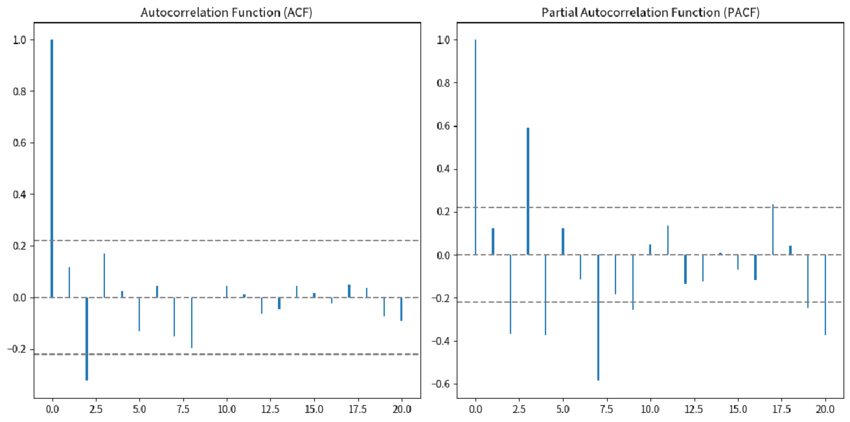
\includegraphics[width=0.5\linewidth]{sampleacf.png}
    \end{center}
    \item Some examples of model-implied ACF and PACF, namely AR(1), AR(1), MA(1), AR(2), and ARMA(1,1):
    \begin{center}
        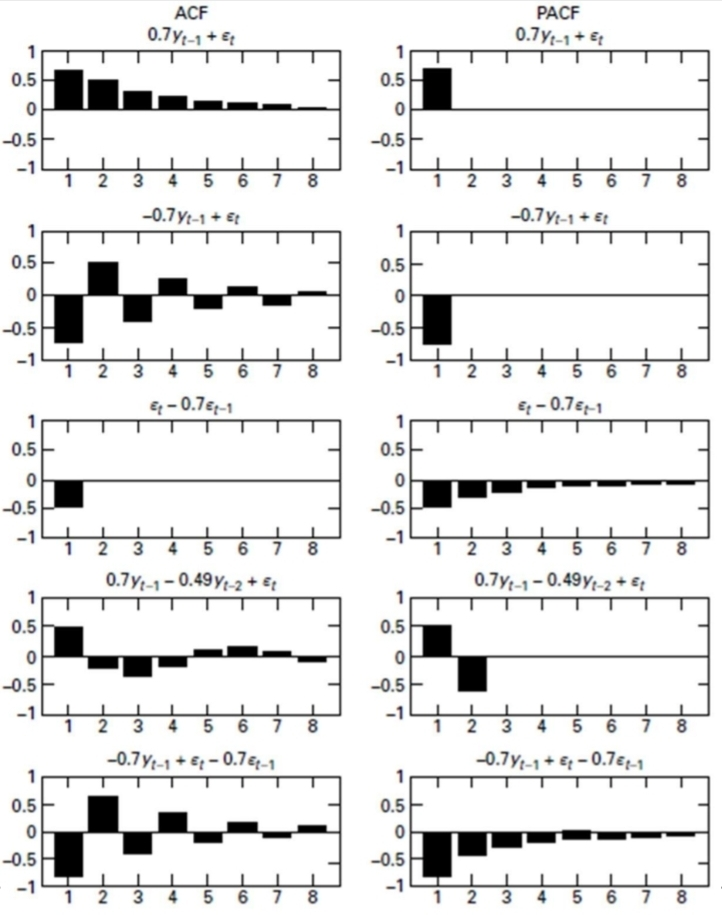
\includegraphics[width=0.5\linewidth]{acf.jpg}
    \end{center}

    \item After fitting a model, we need to check whether it fulfills the assumption that the residuals \(\hat{u}_t = y_t - \hat{y}_t\) are white noises.
    \item Both \textbf{Box-Pierce} and \textbf{Ljung-Box test} test for the following:
    \begin{itemize}
        \item \(H_0\): The first \(m\) autocorrelations are zero (\(\rho_1 = \dots = \rho_m = 0\)).
        \item \(H_1\): At least one autocorrelation is not zero.
    \end{itemize}
    \item Then, we can look at the Q-statistic (\(Q = T\sum_{j=1}^m \hat{\rho}_j^2 \sim \chi^2_{m-p}\) for Box-Pierce, \(Q = T(T+2)\sum_{j=1}^m \frac{\hat{\rho}_j^2}{T-j} \sim \chi^2_{m-p}\) for Ljung-Box) and the corresponding p-value to determine whether \(H_0\) is rejected. If \(H_0\) is rejected, then the residuals are not white noises, which implies the model is not good enough.
\end{itemize}

\subsection{Forecasting with AR Model}

\begin{itemize}
    \item We want to get the \textbf{j-step forecast} for \(y_{t+j}\), given an \textbf{information set} \(I_t = \{y_1, \dots, y_t, u_1, \dots, u_t\}\).
    \item Consider an AR(1): \(y_t = c + \phi y_{t-1} + u_t\).
    \item Note that \(\mathbb{E}[y_{t-j} \mid I_t] = y_{t-j}\) for all \(j \ge 0\), and \(\mathbb{E}[u_{t+j} \mid I_t] = 0\) for all \(j > 0\).
    \item Then:
    \begin{align*}
    \mathbb{E}[y_{t+1} \mid I_t] &= \mathbb{E}[c + \phi y_{t} + u_{t+1} \mid I_t] = c + \phi y_{t} \\
    \mathbb{E}[y_{t+2} \mid I_t] &= \mathbb{E}[c + \phi y_{t+1} + u_{t+2} \mid I_t] = c + \phi \mathbb{E}[y_{t+1} \mid I_t] = (1+\phi)c + \phi^2y_t \\
    % \mathbb{E}[y_{t+2} \mid I_t] &= \mathbb{E}[\mathbb{E}[y_{t+2} \mid I_{t+1}] \mid I_t] = \mathbb{E}[c + \phi y_{t+1} + u_{t+2} \mid I_t] = c + \phi \mathbb{E}[y_{t+1} \mid I_t] = (1+\phi)c + \phi^2y_t
    \end{align*}
    It follows that:
    \[
    \mathbb{E}[y_{t+j} \mid I_t] = c\sum_{k=0}^{j-1}\phi^k + \phi^jy_t
    \]
    \item The \textbf{long term forecast} is equivalent to the \textbf{unconditional forecast}:
    \[
    \mathbb{E}[y_t] = \lim_{j \to \infty}\mathbb{E}[y_{t+j} \mid I_t] = c\sum_{k=0}^{\infty}\phi^k = \frac{c}{1-\phi}
    \]
    Alternatively, we can also directly solve algebraically, using the property \(\mathbb{E}[y_t] = \mathbb{E}[y_{t-1}]\):
    \[
        \mathbb{E}[y_t] = \mathbb{E}[c + \phi y_{t-1} + u_t] = c + \phi \mathbb{E}[y_t] \implies \mathbb{E}[y_t] = \frac{c}{1-\phi} 
    \]
    \item What is the forecast error?
    \begin{align*}
        e_t(1) &= y_{t+1} - \mathbb{E}[y_{t+1} \mid I_t] = (c + \phi y_{t} + u_{t+1}) - (c + \phi y_{t}) = u_{t+1} \\
        e_t(2) &= y_{t+2} - \mathbb{E}[y_{t+2} \mid I_t] = (c + \phi y_{t+1} + u_{t+2}) - (c + \phi \mathbb{E}[y_{t+1} \mid I_t]) = u_{t+2} + \phi (y_{t+1} - \mathbb{E}[y_{t+1} \mid I_t]) = u_{t+2} + \phi u_{t+1}
    \end{align*}
    It follows that:
    \[
    e_t(j) = \sum_{k=1}^{j} \phi^{j-k}u_{t+k}
    \]
    \item What is the variance of the forecast error?
    \[
    \Var(e_t(j)) = \Var(\sum_{k=1}^{j} \phi^{j-k}u_{t+k}) = \sum_{k=1}^{j} \phi^{2(j-k)}\Var(u_t) = \sum_{k=1}^{j} \phi^{2(j-k)} \sigma^2
    \]
    Let \(m=j-k\), then \(\sum_{k=1}^{j} \phi^{2(j-k)} \sigma^2 = \sum_{m=0}^{j-1} \phi^{2m} \sigma^2\). As \(j \to \infty\):
    \[
    \lim_{j \to \infty}\Var(e_t(j)) = \sum_{m=0}^{\infty} \phi^{2m} \sigma^2 = \frac{\sigma^2}{1-\phi^2} = \Var(y_t)
    \]
    \item If \(u_t\) is i.i.d. normal, then \(e_t(j)\) is also normal:
    \[
    e_t(j) \mid I_t \sim \mathcal{N}(0, \Var(e_t(j)))
    \]
    By standardization:
    \[
    \mathbb{P}\left(\left|\frac{e_t(j)}{\sqrt{\Var(e_t(j))}}\right| < 1.96 \mid I_t\right) = \mathbb{P}\left(\left|\frac{y_{t+j} - \mathbb{E}[y_{t+j} \mid I_t] }{\sqrt{\Var(e_t(j))}}\right| < 1.96 \mid I_t\right) = 0.95
    \]
    Hence, the 95\% confidence interval for \(y_{t+j}\) is:
    \[
    y_{t+j} \in \left[\mathbb{E}[y_{t+j} \mid I_t] \pm 1.96 \sqrt{\Var(e_t(j))}\right]
    \]

    \item If the model is estimated using all data \(\{y_1, \dots, y_T\}\), then there can be two kinds of forecasting:
    \begin{enumerate}
        \item \textbf{In-sample forecasting}: \(\mathbb{E}[y_{t+j} \mid I_t]\), where \(t+j \le T\). This serves as \textbf{backtesting} to see if the model aligns with the actual data in the past.
        \item \textbf{Out-of-sample forecasting}: \(\mathbb{E}[y_{T+j} \mid I_T]\), where \(j > 0\). The actual forecasting we want to make.
    \end{enumerate}
    \begin{itemize}
        \item In practice, for better evaluation, we can separate the data: Use \(\{y_1, \dots, y_t\}\) as the \textbf{training data} to estimate the model, and use \(\{y_{t+1}, \dots, y_T\}\) as the \textbf{test data} to evaluate the performance.
    \end{itemize}

    \begin{center}
        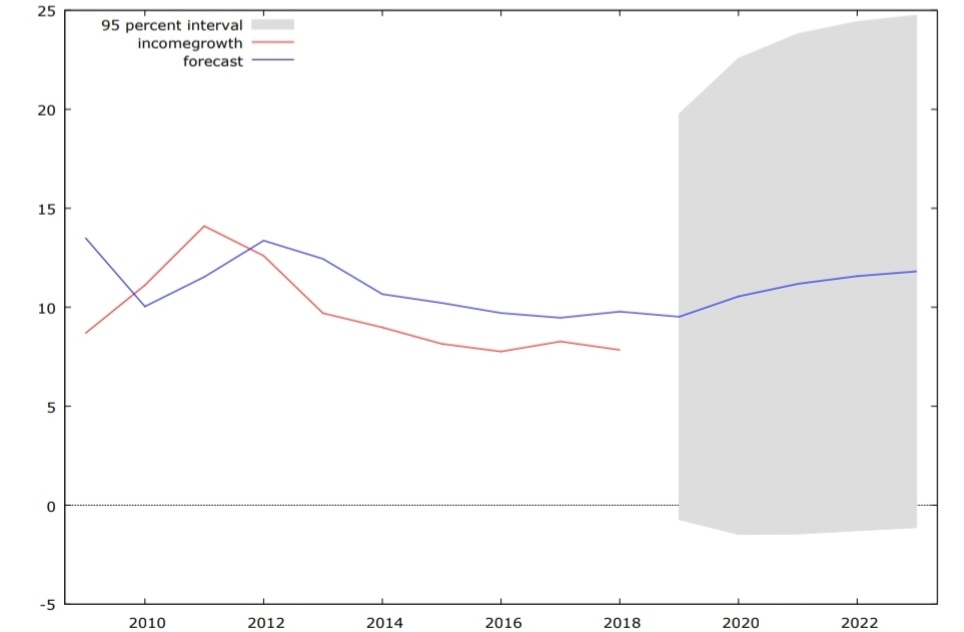
\includegraphics[width=0.5\linewidth]{forecast.jpg}
    \end{center}
\end{itemize}

\subsection{MA Model}

\begin{itemize}
    \item A \textbf{moving average} model with order \(q\), MA(\(q\)), is defined as:
    \[
    y_t = \mu + u_t + \sum_{j=1}^q \theta_j u_{t-j} = \mu + u_t + \theta_1 u_{t-1} + \dots + \theta_q u_{t-q}
    \]
    where \(u_t\) is a white noise process.
    \item Why is it called a moving average?
    \item An example:
    \begin{itemize}
        \item Consider tossing a fair coin and let \(u_t\) denote the payoff at toss \(t\), \$1 if wins and -\$1 if loses. Note that \(u_t\) fulfills all three conditions for a white noise. Let \(y_t\) be the average payoff on the last 4 tosses.
        \[
        y_t = \frac{u_t+u_{t-1}+u_{t-2}+u_{t-3}}{4} = 0.25u_t+0.25u_{t-1}+0.25u_{t-2}+0.25u_{t-3}
        \]
    \end{itemize}
    \item An MA(q) is always stationary, because:
    \[
    \Var(y_t) = \Var(\mu + u_t + \theta_1 u_{t-1} + \dots + \theta_q u_{t-q})  = \Var(u_t) + \theta_1^2\Var(u_{t-1}) + \dots + \theta_q^2\Var(u_{t-q}) = (1+\sum_{j=1}^q\theta_j^2)\sigma^2
    \]
    \item Consider an MA(1) with zero mean: \(y_t = u_t + \theta u_{t-1}\). Again, we have \(\gamma_j = \mathbb{E}[y_ty_{t-j}]\). We derive the ACF by the Yule-Walker equations.
    \begin{align*}
        y_ty_{t-j} &= u_ty_{t-j} + \theta u_{t-1}y_{t-j}\\
        \mathbb{E}[y_ty_{t-j}] &= \mathbb{E}[u_ty_{t-j}] + \theta \mathbb{E}[u_{t-1}y_{t-j}] \\
        &= \mathbb{E}[u_t(u_{t-j} + \theta u_{t-j-1})] + \theta \mathbb{E}[u_{t-1}(u_{t-j} + \theta u_{t-j-1})] \\
        &= \mathbb{E}[u_tu_{t-j}] + \theta\mathbb{E}[u_tu_{t-j-1}] + \theta\mathbb{E}[u_{t-1}u_{t-j}] + \theta^2\mathbb{E}[u_{t-1}u_{t-j-1}]
    \end{align*}
    Note that \(\mathbb{E}[u_t^2] = \sigma^2\) and \(\mathbb{E}[u_tu_{t-j}] = 0\) for all \(j\ne0\) by definition of white noise. Then, for \(j=0\):
    \[
    \gamma_0 = \mathbb{E}[y_t^2] = (1+\theta^2)\sigma^2
    \]
    For \(j=1\):
    \[
    \gamma_1 = \mathbb{E}[y_ty_{t-1}] = \theta\sigma^2 
    \]
    And \(\gamma_j = 0\) for all \(j \ge 2\). Dividing both sides by \(\gamma_0\), the ACF is simply:
    \[
    \rho_j = \frac{\gamma_j}{\gamma_0} =
    \begin{cases}
        \frac{\theta}{1+\theta^2} &\text{if } j=1 \\
        0 & \text{otherwise}
    \end{cases}
    \]
    \item The PACF for an MA(\(q\)) is a long tail (persists infinitely), since it is equivalent to an AR(\(\infty\)) (under certain conditions, proof omitted).
    \item Conversely, an AR(\(p\)) is equivalent to an MA(\(\infty\)). For example, for an AR(1) :
    \[
    y_t = c+ \phi y_{t-1} + u_t = c+ \phi (c+ \phi y_{t-2} + u_{t-1}) + u_t = \dots = \frac{c}{1-\phi} + \sum_{j=0}^\infty \phi^j u_{t-j}
    \]
    \item This is the reason why their ACF and PACF have opposite shapes.
\end{itemize}

\subsection{ARMA Model}

\begin{itemize}
    \item An \textbf{autoregressive moving average model} with order (\(p,q\)), ARMA(\(p,q\)), is defined as:
    \[
    y_t = c + \sum_{i=1}^p \phi_i y_{t-i} + u_t + \sum_{j=1}^q \theta_j u_{t-j}
    \]
    \item Stationarity only depends on the AR coefficients with the same condition: \(|\phi| < 1\) for \(p=1\), all roots for the characteristic equation lie within a unit circle for \(p \ge 1\).
    \item Wold’s decomposition theorem: Any stationary series has an MA(\(\infty\)) representation, including ARMA(\(p,q\)), AR(\(p\)), MA(\(q\)).
    \item Yule-Walker equations for an ARMA(1,1) with zero mean: \(y_t = \phi y_{t-1} + u_t + \theta u_{t-1}\),
    \begin{align*}
        y_t y_{t-j} &= \phi y_{t-1} y_{t-j} + u_t y_{t-j} + \theta u_{t-1}y_{t-j} \\
        \mathbb{E}[y_t y_{t-j}] &= \phi \mathbb{E}[y_{t-1} y_{t-j}] + \mathbb{E}[u_t y_{t-j}] + \theta \mathbb{E}[u_{t-1}y_{t-j}]
    \end{align*}
    Note that \(\mathbb{E}[y_{t-1} y_{t-j}] = \gamma_{j-1}\), \(\mathbb{E}[u_t y_{t}] = \sigma^2\), and \(\mathbb{E}[u_t y_{t-j}] = 0\) for \(j>0\). Also,
    \[
    \mathbb{E}[u_{t-1} y_t] = \mathbb{E}[u_{t-1} (\phi y_{t-1} + u_t + \theta u_{t-1})] = (\phi+\theta)\sigma^2
    \]
    Then, we have:
    \[
    \begin{cases}
        \gamma_0 = \phi \gamma_1 + \sigma^2 + \theta (\phi+\theta)\sigma^2 \\
        \gamma_1 = \phi \gamma_0 + \theta \sigma^2 \\
        \gamma_j = \phi \gamma_{j-1} &\text{for all } j\ge2
    \end{cases}
    \]
    Solving for the first two equations, we can get \(\gamma_0 = \frac{1+\theta^2+2\phi\theta}{1-\phi^2}\sigma^2\) and \(\gamma_1 = \frac{(1+\phi\theta)(\phi+\theta)}{1-\phi^2}\sigma^2\). Hence, \(\rho_1 = \frac{(1+\phi\theta)(\phi+\theta)}{1+\theta^2+2\phi\theta}\) and \(\rho_j = \phi \rho_{j-1}\) for all \(j \ge 2\).
\end{itemize}

\subsection{Model Selection}

\begin{itemize}
    \item While we can choose the parameters (\(p,q\)) by looking at the sample ACF and PACF, often times we still have multiple candidates.
    \item We can use something called \textbf{information criteria}, for example:
    \begin{align*}
        \text{AIC} &= 2\ln(\hat{\delta}) + \frac{2k}{T} \\
        \text{SBIC} &= 2\ln(\hat{\delta}) + \frac{k\ln(T)}{T} \\
        \text{HBIC} &= 2\ln(\hat{\delta}) + \frac{2k\ln(\ln(T))}{T}
    \end{align*}
    where \(\hat{\delta}\) is the error (e.g. SER, RMSE) and \(k\) is the number of parameters (i.e. \(c, \phi_i, \theta_j\)).
    \item Other things being equal, we should choose a model with the smallest information criteria, which gives us a model with the best trade-off between bias (underfitting) and variance (overfitting).
\end{itemize}

\section{Modeling Conditional Variance: ARCH and GARCH Models}

\subsection{Model Specifications}

\begin{itemize}
    % \item Previously, we assumed that the \textbf{conditional variance} of the error term is constant: \(\Var(u_{t+j} \mid I_t) = \sigma^2\) (\textbf{homoscedastic}). However, it is often \textbf{heteroscedastic} instead.
    \item So far we have mainly been using the \textbf{unconditional variance} of the error term: \(\Var(u_t) = \sigma^2\), but observe that when we compute the variance of a conditional forecast, say, for an ARMA(1,1):
    \[
    \Var(y_{t+1} \mid I_t) = \Var(c + \phi y_t + u_{t+1} + \theta u_t \mid I_t) = \Var(u_{t+1} \mid I_t)
    \]
    we have to make use of the \textbf{conditional variance} \(\Var(u_{t+1} \mid I_t)\).
    \item It is natural to think that it is constant: \(\Var(u_{t+1} \mid I_t) = \Var(u_t) = \sigma^2\) (\textbf{homoscedastic}), but is it really the case?
    \item For example, stock returns are often \textbf{heteroscedastic} and exhibit the following features:
    \begin{enumerate}
        \item Volatility cluster: If the volatility in period \(t-1\) is high, then it's more likely that period \(t\) is also volatile.
        \item Fat tails: The probability of having extremely high or extremely low returns (kurtosis) is higher than usual.
        \item Asymmetry: Negative shocks at period \(t-1\) have a stronger effect on period \(t\).
    \end{enumerate}
    \item In addition to the white noise assumptions for \(u_t\), we strengthen it with one more condition:
    \[
    \mathbb{E}[u_t \mid I_{t-1}] = 0
    \]
    which makes it a \textbf{martingale difference sequence}.
    \item Then, we can obtain:
    \[
    \Var(y_t \mid I_{t-1}) = \Var(u_t \mid I_{t-1}) = \mathbb{E}[u_t^2 \mid I_{t-1}] - \mathbb{E}[u_t \mid I_{t-1}]^2 = \mathbb{E}[u_t^2 \mid I_{t-1}]
    \]
    To model the volatility cluster, we may assume:
    \[
    \mathbb{E}[u_t^2 \mid I_{t-1}] = \alpha_0 + \sum_{j=1}^q \alpha_j u_{t-j}^2
    \]
    \item One idea is using an AR model:
    \[
    u_t^2 = \alpha_0 + \sum_{j=1}^q \alpha_j u_{t-j}^2 + v_t
    \]
    where \(\mathbb{E}[v_t \mid I_{t-1}]=0\).
    \item Engle (1982) proposed the \textbf{autoregressive conditional heteroskedasticity} model, ARCH(\(q\)), instead, defined as:
    \[
    u_t = v_t\sqrt{h_t}, \;h_t = \alpha_0 + \sum_{j=1}^q \alpha_j u_{t-j}^2
    % u_t = v_t\sqrt{\alpha_0 + \sum_{j=1}^q \alpha_j u_{t-j}^2}
    \]
    where \(\mathbb{E}[v_t \mid I_{t-1}]=0\) and \(\mathbb{E}[v_t^2 \mid I_{t-1}]=1\). For example, we can assume \(v_t \overset{\text{i.i.d.}}{\sim} \mathcal{N}(0,1)\).
    \item Note that \(u_t\) and \(h_t\) are uncorrelated. Then, we can derive some features:
    \begin{itemize}
        \item Volatility cluster: (Note that since \(u_{t-j} \in I_{t-1}\) for all \(j\ge1\), \(h_t \in I_{t-1}\).)
        \[
        \mathbb{E}[u_t^2 \mid I_{t-1}] = \mathbb{E}[v_t^2 h_t \mid I_{t-1}] = \mathbb{E}[v_t^2 \mid I_{t-1}] \cdot h_t = h_t
        \]
        Since we are interested in the conditional variance, \(\Var(y_t \mid I_{t-1}) = \mathbb{E}[u_t^2 \mid I_{t-1}] = h_t\) means we are essentially modeling \(h_t\).
        \item Martingale difference:
        \[
            \mathbb{E}[u_t \mid I_{t-1}] = \mathbb{E}[v_t\sqrt{h_t} \mid I_{t-1}] = \mathbb{E}[v_t \mid I_{t-1}] \mathbb{E}[\sqrt{h_t} \mid I_{t-1}] = 0
        \]
        \item No serial correlation:
        \[
            \mathbb{E}[u_tu_{t-j} \mid I_{t-1}] = \mathbb{E}[u_t \mid I_{t-1}] \cdot u_{t-j} = 0 
        \]
        \item Stationary (Mean reversion): (Note that the unconditional variance \(\mathbb{E}[u_t^2] = \mathbb{E}[u_{t-j}^2]\).)
        \[
            \mathbb{E}[u_t^2] = \mathbb{E}[\mathbb{E}[u_t^2 \mid I_{t-1}]] = \mathbb{E}[\alpha_0 + \sum_{j=1}^q \alpha_j u_{t-j}^2] = \alpha_0 + \sum_{j=1}^q \alpha_j \mathbb{E}[u_t^2] \implies \mathbb{E}[u_t^2] = \frac{\alpha_0}{1 - \sum_{j=1}^q \alpha_j}
        \]
        Therefore, \(u_t\) is stationary only if \(\sum_{j=1}^q \alpha_j < 1\).
        \item We can also verify that \(u_t\) is still a white noise process, which is compatible with an ARMA(\(p,q\)).
    \end{itemize}

    \item We also have the generalized ARCH, GARCH(\(p,q\)), defined as:
    \[
    u_t = v_t\sqrt{h_t}, \;h_t = \alpha_0 + \sum_{i=1}^q \alpha_i u_{t-i}^2 + \sum_{j=1}^p \beta_j h_{t-j}
    \]
    where \(\mathbb{E}[v_t \mid I_{t-1}]=0\) and \(\mathbb{E}[v_t^2 \mid I_{t-1}]=1\).
    \item In a GARCH model, conditional variance depends not only on past shocks, but also on past variances. Thus, it captures persistent volatility more effectively. For example, modeling highly persistent volatility often requires an ARCH($q$) with many lags, whereas a GARCH(1,1) suffices.
    \item GARCH also has similar features, for example:
    \begin{itemize}
        \item Conditional volatility:
        \[
        \mathbb{E}[u_t^2 \mid I_{t-1}] = \mathbb{E}[v_t^2 h_t \mid I_{t-1}] = \mathbb{E}[v_t^2 \mid I_{t-1}] \cdot h_t = h_t
        \]
        \item For unconditional volatility, first note that:
        \[
        \mathbb{E}[u_t^2] = \mathbb{E}[\mathbb{E}[u_t^2 \mid I_{t-1}]] = \mathbb{E}[h_t]
        \]
        Also given that \(\mathbb{E}[u_t^2] = \mathbb{E}[u_{t-j}^2]\) and \(\mathbb{E}[h_t] = \mathbb{E}[h_{t-j}]\), we can get:
        \[
        \mathbb{E}\left[\alpha_0 + \sum_{i=1}^q \alpha_i u_{t-i}^2 + \sum_{j=1}^p \beta_j h_{t-j}\right] = \alpha_0 + \sum_{i=1}^q \alpha_i \mathbb{E}[u_t^2] + \sum_{j=1}^p \beta_j \mathbb{E}[h_t] = \alpha_0 + \sum_{i=1}^q \alpha_i \mathbb{E}[u_t^2] + \sum_{j=1}^p \beta_j \mathbb{E}[u_t^2]
        \]
        Therefore:
        \[
        \mathbb{E}[u_t^2] = \frac{\alpha_0}{1 - \sum_{i=1}^q \alpha_i - \sum_{j=1}^p \beta_j}
        \]
        \item Hence, \(u_t\) is stationary only if \(\sum_{i=1}^q \alpha_i + \sum_{j=1}^p \beta_j < 1\).
    \end{itemize}
    \item To model asymmetry, we may use a GJR-GARCH model, defined as:
    \[
    u_t = v_t\sqrt{h_t}, \; h_t = \alpha_0 + \sum_{i=1}^q (\alpha_i + \gamma_i \mathbb{I}(u_{t-i}<0)) u_{t-i}^2 + \sum_{j=1}^p \beta_j h_{t-j}
    \]
    where \(\mathbb{I}(u_{t-i}<0) = 1\) if \(u_{t-i}<0\) and 0 otherwise.
\end{itemize}

\subsection{Forecasting with ARCH and GARCH}

\begin{itemize}
    \item Consider an ARCH(1):
    \[
    u_t = v_t\sqrt{\alpha_0 + \alpha_1 u_{t-1}^2}
    \]
    We will make use of the generalized law of iterated expectation:
    \[
    \mathbb{E}[x_t \mid I_{t-j}] =  \mathbb{E}[\mathbb{E}[x_t \mid I_{t-i}]  \mid I_{t-j}]
    \]
    if \(j \ge i\). Since \(I_{t-j}\) is a smaller information set (\(I_{t-j} \subset I_{t-i}\) ), it dominates the expectation.

    First:
    \[
    \mathbb{E}[u_{t+1}^2 \mid I_t] = \mathbb{E}[v_{t+1}^2 (\alpha_0 + \alpha_1 u_t^2) \mid I_t] = \mathbb{E}[v_{t+1}^2 \mid I_{t}] \cdot (\alpha_0 + \alpha_1 u_t^2) = \alpha_0 + \alpha_1 u_t^2
    \]
    Thus, we know that:
    \[
    \mathbb{E}[u_{t+2}^2 \mid I_{t+1}] = \alpha_0 + \alpha_1 u_{t+1}^2
    \]
    Then:
    \[
    \mathbb{E}[u_{t+2}^2 \mid I_t] = \mathbb{E}[\mathbb{E}[u_{t+2}^2 \mid I_{t+1}]  \mid I_{t}] =  \mathbb{E}[\alpha_0 + \alpha_1 u_{t+1}^2 \mid I_{t}] = \alpha_0 + \alpha_1 \mathbb{E}[u_{t+1}^2 \mid I_t]
    \]
    This gives us a recurrence relation:
    \[
    \mathbb{E}[u_{t+j}^2 \mid I_t] = \alpha_0 + \alpha_1 \mathbb{E}[u_{t+j-1}^2 \mid I_t]
    \]
    which can be solved by iterated substitution till we reach \(j=1\).
    \item Similarly, for a GARCH(1,1):
    \[
    u_t = v_t\sqrt{h_t}, \;h_t = \alpha_0 + \alpha_1 u_{t-1}^2 + \beta h_{t-1}
    \]
    Again, note that \(h_{t+1} \in I_t\). First:
    \[
    \mathbb{E}[u_{t+1}^2 \mid I_t] = \mathbb{E}[v_{t+1}^2 h_{t+1} \mid I_t] = \mathbb{E}[v_{t+1}^2 \mid I_{t}] \cdot h_{t+1} = h_{t+1}
    \]
    Thus, we know that:
    \[
    \mathbb{E}[u_{t+2}^2 \mid I_{t+1}] = h_{t+2}
    \]
    Then:
    \[
    \mathbb{E}[u_{t+2}^2 \mid I_t] = \mathbb{E}[\mathbb{E}[u_{t+2}^2 \mid I_{t+1}]  \mid I_{t}] = \mathbb{E}[h_{t+2} \mid I_{t}] = \mathbb{E}[\alpha_0 + \alpha_1 u_{t+1}^2 + \beta h_{t+1} \mid I_{t}]
    \]
    Given that \(\mathbb{E}[u_{t+1}^2 \mid I_t] = h_{t+1} = \mathbb{E}[h_{t+1} \mid I_t]\), we have:
    \[
    \mathbb{E}[\alpha_0 + \alpha_1 u_{t+1}^2 + \beta h_{t+1} \mid I_{t}] = \alpha_0 + \alpha_1 \mathbb{E}[u_{t+1}^2 \mid I_t] + \beta \mathbb{E}[u_{t+1}^2 \mid I_t] = \alpha_0 + (\alpha_1 + \beta) \mathbb{E}[u_{t+1}^2 \mid I_t]
    \]
    It follows that:
    \[
    \mathbb{E}[u_{t+j}^2 \mid I_t] = \alpha_0 + (\alpha_1 + \beta) \mathbb{E}[u_{t+j-1}^2 \mid I_t]
    \]
\end{itemize}

\subsection{Model Fitting and Diagnostics}

\begin{itemize}
    \item In practice, the error terms we want to model are derived from the residuals of another model. For example, a full model can be an AR(1)-GARCH(1,1):
    \begin{align*}
        y_t &= c + \phi y_{t-1} + u_t \\
        u_t &= v_t \sqrt{h_t} \\
        h_t &= \alpha_0 + \alpha_1 u^2_{t-1} + \beta h_{t-1}
    \end{align*}
    where \(\mathbb{E}[v_t \mid I_{t-1}] = 0\) and \(\mathbb{E}[v_t^2 \mid I_{t-1}] = 1\).

    \item To choose the hyperparameters (\(p,q\)) for ARCH or GARCH, one can look at the ACF and PACF of \(\hat{u}_t^2\), which is an estimator for \(h_t\). Information criteria are also useful.

    \item After fitting and estimating the parameters \(c, \phi, \alpha_0, \alpha_1, \beta\), we need to conduct autocorrelation test (Box–Pierce/Ljung–Box) for two items to ensure they have no autocorrelation:
    \begin{itemize}
        \item \(\hat{v}_t = \frac{\hat{u}_t}{\sqrt{\hat{h}_t}}\): If \(v_t\) is not a white noise, then \(u_t\) is not a white noise, which violates the AR assumption.
        \item \(\hat{v}_t^2 = \frac{\hat{u}^2_t}{\hat{h}_t}\): If \(\hat{v}_t^2\) has serial autocorrelations, then there is remaining conditional heteroskedasticity that the GARCH cannot capture.
    \end{itemize}
\end{itemize}

\section{Modeling Multivariate Data: VAR Model}

\subsection{Structural VAR}

\begin{itemize}
    \item In ARMA models, we only focus on one variable \(y_t\). However, what if we have multiple time series variables that are dependent on each other?
    \item For example, suppose \(y_{1t}\) follows AR(1), so it is dependent on \(y_{1,t-1}\). On top of that, it is also dependent on another variable, \(y_{2t}\) and \(y_{2,t-1}\), where \(y_{2t}\) follows a symmetrical relationship.
    \begin{align*}
        y_{1t} &= c_1 + \beta y_{2t} + \phi_{11}y_{1,t-1} + \phi_{12}y_{2,t-1} + \varepsilon_{1t} \\
        y_{2t} &= c_2 + \gamma y_{1t} + \phi_{21}y_{1,t-1} + \phi_{22}y_{2,t-1} + \varepsilon_{2t}
    \end{align*}
    \item \(\varepsilon_{1t}\) and \(\varepsilon_{2t}\) are white noises and independent \textbf{structural shocks}: \(\Cov(\varepsilon_{1t}, \varepsilon_{2t}) = 0\).
    \item However, if \(\beta, \gamma \ne 0\), then \(\Cov(y_{1t}, \varepsilon_{2t}), \Cov(y_{2t}, \varepsilon_{1t}) \ne 0\) by a chain of reaction: \(\varepsilon_{1t} \rightarrow y_{1t} \rightarrow y_{2t} \rightarrow y_{1t} \rightarrow y_{2t} \dots\)
    \item Specifically:
    \begin{align*}
    \Cov(y_{1t}, \varepsilon_{2t}) &= \Cov(c_1 + \beta y_{2t} + \phi_{11}y_{1,t-1} + \phi_{12}y_{2,t-1} + \varepsilon_{1t}, \varepsilon_{2t}) \\
    &= \beta \Cov(y_{2t}, \varepsilon_{2t}) \\
    &= \beta \Cov(c_2 + \gamma y_{1t} + \phi_{21}y_{1,t-1} + \phi_{22}y_{2,t-1} + \varepsilon_{2t}, \varepsilon_{2t}) \\
    &= \beta\gamma \Cov(y_{1t}, \varepsilon_{2t}) + \beta \Var(\varepsilon_{2t}) \\
    \implies \Cov(y_{1t}, \varepsilon_{2t}) &= \frac{\beta \Var(\varepsilon_{2t})}{1-\beta\gamma}
    \end{align*}
    By symmetry, we can get:
    \[
    \Cov(y_{2t}, \varepsilon_{1t}) = \frac{\gamma \Var(\varepsilon_{1t})}{1-\beta\gamma}
    \]
    \item Since the regressor is correlated with the error term, OLS fails to estimate this model.
    \item We call this form of model a \textbf{structural VAR} (vector autoregression) or \textbf{SVAR}. This can also be represented in a vector-matrix form:
    \[
    \begin{bmatrix} y_{1t} \\ y_{2t} \end{bmatrix} =
    \begin{bmatrix} c_1 \\ c_2 \end{bmatrix} +
    \begin{bmatrix} 0 & \beta \\ \gamma & 0 \end{bmatrix}
    \begin{bmatrix} y_{1t} \\ y_{2t} \end{bmatrix} +
    \begin{bmatrix} \phi_{11} & \phi_{12} \\ \phi_{21} & \phi_{22} \end{bmatrix}
    \begin{bmatrix} y_{1,t-1} \\ y_{2,t-1} \end{bmatrix} +
    \begin{bmatrix} \varepsilon_{1t} \\ \varepsilon_{2t} \end{bmatrix}
    \]
\end{itemize}

\subsection{Reduced-form VAR}

\begin{itemize}
    \item For the model to be able to be estimated by OLS, we need to get rid of the \(y_{jt}\) term in the equation of \(y_{it}\) to obtain a \textbf{reduced-form VAR}.
    \item For example:
    \begin{align*}
        y_{1t} &= c_1 + \beta y_{2t} + \phi_{11}y_{1,t-1} + \phi_{12}y_{2,t-1} + \varepsilon_{1t} \\
        &= c_1 + \beta (c_2 + \gamma y_{1t} + \phi_{21}y_{1,t-1} + \phi_{22}y_{2,t-1} + \varepsilon_{2t}) + \phi_{11}y_{1,t-1} + \phi_{12}y_{2,t-1} + \varepsilon_{1t} \\
        &= (c_1 + \beta c_2) + \beta \gamma y_{1t} + (\phi_{11} + \beta \phi_{21}) y_{1,t-1} + (\phi_{12} + \beta \phi_{22}) y_{2,t-1} + (\varepsilon_{1t} + \beta \varepsilon_{2t}) \\
        \implies y_{1t} &= \frac{c_1 + \beta c_2}{1-\beta\gamma} + \frac{\phi_{11} + \beta \phi_{21}}{{1-\beta\gamma}} y_{1,t-1} + \frac{\phi_{12} + \beta \phi_{22}}{1-\beta\gamma} y_{2,t-1} + \frac{\varepsilon_{1t} + \beta \varepsilon_{2t}}{1-\beta\gamma}
    \end{align*}
    By symmetry:
    \[
    y_{2t} = \frac{c_2 + \gamma c_1}{1-\beta\gamma} + \frac{\phi_{21} + \gamma \phi_{11}}{{1-\beta\gamma}} y_{1,t-1} + \frac{\phi_{22} + \gamma \phi_{12}}{1-\beta\gamma} y_{2,t-1} + \frac{\varepsilon_{2t} + \gamma \varepsilon_{1t}}{1-\beta\gamma}
    \]
    Let \(e_{1t} = \frac{\varepsilon_{1t} + \beta \varepsilon_{2t}}{1-\beta\gamma}\) and \(e_{2t} = \frac{\varepsilon_{2t} + \gamma \varepsilon_{1t}}{1-\beta\gamma}\), since they are uncorrelated to any regressor (\(y_{1,t-1}\), \(y_{2,t-1}\)), these two can be estimated by OLS. However, while \(\Cov(\varepsilon_{1t}, \varepsilon_{2t}) =0 \), now \(\Cov(e_{1t}, e_{2t}) \ne 0\).

    \item In vector-matrix form:
    \begin{align*}
        \begin{bmatrix} 1 & 0 \\ 0 & 1 \end{bmatrix}
        \begin{bmatrix} y_{1t} \\ y_{2t} \end{bmatrix} &=
        \begin{bmatrix} c_1 \\ c_2 \end{bmatrix} +
        \begin{bmatrix} 0 & \beta \\ \gamma & 0 \end{bmatrix}
        \begin{bmatrix} y_{1t} \\ y_{2t} \end{bmatrix} +
        \begin{bmatrix} \phi_{11} & \phi_{12} \\ \phi_{21} & \phi_{22} \end{bmatrix}
        \begin{bmatrix} y_{1,t-1} \\ y_{2,t-1} \end{bmatrix} +
        \begin{bmatrix} \varepsilon_{1t} \\ \varepsilon_{2t} \end{bmatrix} \\
        \begin{bmatrix} 1 & -\beta \\ -\gamma & 1 \end{bmatrix}
        \begin{bmatrix} y_{1t} \\ y_{2t} \end{bmatrix} &=
        \begin{bmatrix} c_1 \\ c_2 \end{bmatrix} +
        \begin{bmatrix} \phi_{11} & \phi_{12} \\ \phi_{21} & \phi_{22} \end{bmatrix}
        \begin{bmatrix} y_{1,t-1} \\ y_{2,t-1} \end{bmatrix} +
        \begin{bmatrix} \varepsilon_{1t} \\ \varepsilon_{2t} \end{bmatrix} 
    \end{align*}
    We can denote this as:
    \begin{align*}
        \mathbf{A}_0\mathbf{y}_t &= \mathbf{c} + \boldsymbol{\Psi}\mathbf{y}_{t-1} + \boldsymbol{\varepsilon}_t \\
        \mathbf{y}_t &= \mathbf{A}_0^{-1}\mathbf{c} + \mathbf{A}_0^{-1}\boldsymbol{\Psi}\mathbf{y}_{t-1} + \mathbf{A}_0^{-1}\boldsymbol{\varepsilon}_t
    \end{align*}
    Let \(\mathbf{A} = \mathbf{A}_0^{-1}\), then we have \(\mathbf{e}_t = \mathbf{A}\boldsymbol{\varepsilon}_t\).

    \item Recall the variance-covariance matrix of \(\mathbf{x} = [x_1, x_2]^T\) is defined as:
    \[
    \boldsymbol{\Sigma}_\mathbf{x} = \begin{bmatrix} \Var(x_1) & \Cov(x_1, x_2) \\ \Cov(x_2, x_1) & \Var(x_2) \end{bmatrix}
    \]
    If \(\mathbf{y} = \mathbf{A}\mathbf{x}\), then \(\boldsymbol{\Sigma}_\mathbf{y} = \mathbf{A}\boldsymbol{\Sigma}_\mathbf{x}\mathbf{A}^{T}\). Applying this to \(\mathbf{e}_t\), we have \(\boldsymbol{\Sigma}_{\mathbf{e}_t} = \mathbf{A}\boldsymbol{\Sigma}_{\boldsymbol{\varepsilon}_t}\mathbf{A}^{T}\). Since it is not a diagonal matrix, we know \(\Cov(e_{1t}, e_{2t}) \ne 0\).

    \item Comparing SVAR and reduced-form VAR:
    \begin{itemize}
        \item An SVAR carries more economic meanings: variables can have contemporaneous effects on each other, error terms (structural shocks) are independent of each other. However, it cannot be estimated by OLS unless we add some constraints (discuss later).
        \item A reduced-form VAR is more mathematically convenient and flexible to use.
    \end{itemize}

    \item AR and VAR models can be generalized in a \textbf{companion form} which looks like a reduced-form VAR(1), expressed as:
    \[
    \mathbf{y}_t = \mathbf{c} + \boldsymbol{\Phi}\mathbf{y}_{t-1} + \mathbf{e}_t
    \]
    where \(\boldsymbol{\Phi}\) is called the \textbf{companion matrix}. For example:
    \begin{itemize}
        \item For an AR(p):
        \[
        y_t = c + \phi_1 y_{t-1} + \dots + \phi_p y_{t-p} + u_t
        \]
        We may also consider the identities for all \(1 <j < p\):
        \[
        y_{t-j} = 0 + 1 \cdot y_{t-j} + 0
        \]
        Then:
        \[
        \begin{bmatrix} y_t \\ y_{t-1} \\ \vdots \\ y_{t-p+1} \end{bmatrix} = 
        \begin{bmatrix} c \\ 0 \\ \vdots \\ 0 \end{bmatrix} + 
        \begin{bmatrix} \phi_1 & \phi_2 & \dots & \phi_{p-1} & \phi_p \\ 1 & 0 & \dots & 0 & 0 \\ \vdots & \vdots & \ddots & \vdots & \vdots \\ 0 & 0 & \dots & 1 & 0\end{bmatrix}
        \begin{bmatrix} y_{t-1} \\ y_{t-2} \\ \vdots \\ y_{t-p} \end{bmatrix} + 
        \begin{bmatrix} u_t \\ 0 \\ \vdots \\ 0 \end{bmatrix}
        \]
        
        \item Similarly, for a reduced-form VAR(\(p\)):
        \[
        \mathbf{y}_t = \mathbf{c} + \boldsymbol{\Phi}_1 \mathbf{y}_{t-1} + \boldsymbol{\Phi}_2 \mathbf{y}_{t-2} + \dots + \boldsymbol{\Phi}_p \mathbf{y}_{t-p} + \mathbf{e}_t
        \]
        where \(\mathbf{y}_t = [y_{1t}, \dots, y_{nt}]^T\). We can simply stack the vectors and matrices together:
        \[
        \begin{bmatrix} \mathbf{y}_t \\ \mathbf{y}_{t-1} \\ \vdots \\ \mathbf{y}_{t-p+1} \end{bmatrix} = 
        \begin{bmatrix} \mathbf{c} \\ \mathbf{0} \\ \vdots \\ \mathbf{0} \end{bmatrix} + 
        \begin{bmatrix} \boldsymbol{\Phi}_1 & \boldsymbol{\Phi}_2 & \dots & \boldsymbol{\Phi}_{p-1} & \boldsymbol{\Phi}_p \\ \mathbf{I} & \mathbf{0} & \dots & \mathbf{0} & \mathbf{0} \\
        \vdots & \vdots & \ddots & \vdots & \vdots \\ \mathbf{0} & \mathbf{0} & \dots & \mathbf{I} & \mathbf{0}\end{bmatrix} 
        \begin{bmatrix} \mathbf{y}_{t-1} \\ \mathbf{y}_{t-2} \\ \vdots \\ \mathbf{y}_{t-p} \end{bmatrix} + 
        \begin{bmatrix} \mathbf{e}_t  \\ \mathbf{0} \\ \vdots \\ \mathbf{0} \end{bmatrix}
        \]
        \item This form is helpful for checking stationarity: a VAR is stationary if and only if all eigenvalues of the companion matrix lie within a unit circle. One can verify that this aligns with the stationarity condition for AR(\(p\)) defined by the characteristic equation previously.
    \end{itemize}
\end{itemize}

\subsection{Recursive VAR}

\begin{itemize}
    \item An SVAR cannot be estimated by OLS but a reduced-form VAR can. Then, is it possible that we first estimate a reduced-form VAR, and then transform it back to an SVAR?

    \item First, we use a companion form to represent any reduced-form VAR:
    \[
    \mathbf{y}_t = \mathbf{c} + \boldsymbol{\Phi}\mathbf{y}_{t-1} + \mathbf{e}_t
    \]
    We assume that the error term \(\mathbf{e}_t\) is derived from an unknown SVAR, where \(\mathbf{e}_t = \mathbf{A}\boldsymbol{\varepsilon}_t\). Furthermore, for easier calculation later on, we can consider a \textbf{normalized} error term \(\tilde{\boldsymbol{\varepsilon}}_t = \boldsymbol{\Sigma}_{\boldsymbol{\varepsilon}_t}^{-\frac{1}{2}}\boldsymbol{\varepsilon}_t\) such that \(\boldsymbol{\Sigma}_{\tilde{\boldsymbol{\varepsilon}}_t} = \boldsymbol{\Sigma}_{\boldsymbol{\varepsilon}_t}^{-\frac{1}{2}} \boldsymbol{\Sigma}_{\boldsymbol{\varepsilon}_t} (\boldsymbol{\Sigma}_{\boldsymbol{\varepsilon}_t}^{-\frac{1}{2}})^T = \mathbf{I}\). Then, we can rewrite the reduced-form VAR back into an SVAR:
        \[
        \mathbf{y}_t = \mathbf{c} + \boldsymbol{\Phi}\mathbf{y}_{t-1} + \mathbf{e}_t = \mathbf{c} + \boldsymbol{\Phi}\mathbf{y}_{t-1} + \mathbf{A} \boldsymbol{\Sigma}_{\boldsymbol{\varepsilon}_t}^\frac{1}{2} \tilde{\boldsymbol{\varepsilon}}_t = \mathbf{c} + \boldsymbol{\Phi}\mathbf{y}_{t-1} + \tilde{\mathbf{A}} \tilde{\boldsymbol{\varepsilon}}_t
        \]

    To transform back into an SVAR, we now want to find \(\tilde{\mathbf{A}}\) from the reduced-form VAR.

    \begin{itemize}
        \item Also note that since all \(\tilde{\varepsilon}_{j,t}\) have a standard deviation of one, a one-unit increase in \(\tilde{\varepsilon}_{j,t}\) essentially means a one-SD shock in \(y_{j,t}\), which is often more useful than the raw \(\varepsilon_{j,t}\) in analysis.
    \end{itemize}
    
    \item For example, suppose we first estimated a reduced-form VAR and we want to turn it back to an SVAR:
    \[
    \mathbf{y}_t = \boldsymbol{\Phi}\mathbf{y}_{t-1} + \mathbf{e}_t = \boldsymbol{\Phi}\mathbf{y}_{t-1} + \tilde{\mathbf{A}} \tilde{\boldsymbol{\varepsilon}}_t
    \]
    To get \(\tilde{\mathbf{A}}\), we rely on the variance-covariance matrix of \(\mathbf{e}_t\), where:
    \[
        \boldsymbol{\Sigma}_{\mathbf{e}_t} = \tilde{\mathbf{A}}\boldsymbol{\Sigma}_{\tilde{\boldsymbol{\varepsilon}}_t}\tilde{\mathbf{A}}^T = \tilde{\mathbf{A}}\tilde{\mathbf{A}}^T
    \]
    Expanding for a two-variable case, we have:
    \[
    \begin{bmatrix}
        \sigma_1^2 & \sigma_{12} \\ \sigma_{21} & \sigma_2^2
    \end{bmatrix} =
    \begin{bmatrix}
        a_{11} & a_{12} \\ a_{21} & a_{22}
    \end{bmatrix}
    \begin{bmatrix}
        a_{11} & a_{21} \\ a_{12} & a_{22}
    \end{bmatrix}
    \]
    which gives us the following equations:
    \[
    \begin{cases}
        \sigma_1^2 = a_{11}^2 + a_{12}^2 \\
        \sigma_{12} = a_{11}a_{21} + a_{12}a_{22} \\
        \sigma_{21} = a_{11}a_{21} + a_{12}a_{22} \\
        \sigma_2^2 = a_{21}^2 + a_{22}^2
    \end{cases}
    \]
    Because \(\sigma_{12}=\sigma_{21}\), the 2nd and 3rd equations are the same, which means we have 4 variables to be identified but only 3 equations. This is a \textbf{under-identification problem}.
    \item A simple solution: Let \(a_{12}=0\). This way, we assume \(y_1\) is not affected by \(\tilde\varepsilon_{2t}\), i.e. no contemporaneous effect.
    \item Generalizing to more variables, we assume \(\tilde{\mathbf{A}}\) to be a lower triangular matrix to reduce the number of variables. 
    \begin{itemize}
        \item We need to rank the variables from the most exogenous to the least, that is, \(y_{1t}\) is only affected by \(\tilde\varepsilon_{1t}\) contemporaneously, \(y_{2t}\) is only affected by \(\tilde\varepsilon_{1t}\) and \(\tilde\varepsilon_{2t}\), \dots, and \(y_{n,t}\) is affected by all structural shocks.
        \item This form is called a \textbf{recursive VAR}.
        \item The order is usually implied by theory or observations. For example, consider monetary policy: We may assume inflation \(\pi_t\) is given exogenously, unemployment \(u_t\) is affected by it by the Phillips curve, and finally interest rate \(i_t\) is determined by both of these through Taylor rule.
    \end{itemize}
    \item Then, we can solve for:
    \[
    \begin{bmatrix}
        \sigma_1^2 & \sigma_{12} & \dots & \sigma_{1n} \\ \sigma_{21} & \sigma_2^2 & \dots & \sigma_{2n} \\
        \vdots & \vdots & \ddots & \vdots \\
        \sigma_{n1} & \sigma_{n2} & \dots & \sigma_n^2
    \end{bmatrix} =
    \begin{bmatrix}
        a_{11} & 0 & 0 & \dots & 0 \\ a_{21} & a_{22} & 0 & \dots & 0 \\ \vdots & \vdots & \vdots & \ddots & \vdots \\ a_{n1} & a_{n2} & a_{n3} & \dots & a_{nn}
    \end{bmatrix}
    \begin{bmatrix}
        a_{11} & a_{21} & a_{31} & \dots & a_{n1} \\ 0 & a_{22} & a_{32} & \dots & a_{n2} \\ \vdots & \vdots & \vdots & \ddots & \vdots \\ 0 & 0 & 0 & \dots & a_{nn}
    \end{bmatrix}
    \]
    To do this, we can apply a method called \textbf{Cholesky decomposition}, which can decompose a symmetrical matrix \(\mathbf{A}\) as \(\mathbf{A}= \mathbf{L}\mathbf{L}^T\), where \(\mathbf{L}\) is a lower triangular matrix. Applying this, we can obtain \(\boldsymbol{\Sigma}_{\mathbf{e}_t} = \tilde{\mathbf{A}}\tilde{\mathbf{A}}^T\).
\end{itemize} 

\subsection{Impulse Responses}

\begin{itemize}
    \item Sometimes we don't just concern forecasting from the current state, but also what will happen if there is a structural shock.
    \begin{itemize}
        \item For example, we don't just look at how the inflation and unemployment rates will go under the current interest rate, but rather how they will go if the Fed raises the interest rate by one unit today. 
    \end{itemize}
    \item We use a \textbf{impulse response function (IRF)} to represent this, defined as:
    \[
    \text{IRF}(s) = \frac{\partial y_{i, t+s}}{\partial \varepsilon_{j, t}} = \frac{\partial y_{i, t}}{\partial \varepsilon_{j, t-s}}
    \]
    \item For example, for an AR(1), recall that it has an MA(\(\infty\)) representation:
    \[
    y_t = c + \phi y_{t-1} + \varepsilon_t = \frac{c}{1-\phi} + \sum_{j=0}^\infty \phi^j \varepsilon_{t-j}
    \]
    Thus:
    \[
    \text{IRF}(s) = \frac{\partial y_{t}}{\partial \varepsilon_{t-s}} = \phi^s
    \]
    \item In a VAR model, while a shock in \(\varepsilon_{j,t}\) only affects \(y_{j,t}\) in period \(t\), it propagates to all \(y_{i,t+s}\) in the future.


    \item Similar to an AR(1), a VAR(1) also has a VMA(\(\infty\)) representation:
    \[
        \mathbf{y}_t = \mathbf{c} + \boldsymbol{\Phi}\mathbf{y}_{t-1} + \mathbf{e}_t 
        =\mathbf{c} + \boldsymbol{\Phi}(\mathbf{c} + \boldsymbol{\Phi}\mathbf{y}_{t-2} + \mathbf{e}_{t-1}) + \mathbf{e}_t
        = \dots
        = \mathbf{k} + \sum_{j=0}^\infty \boldsymbol{\Phi}^j\mathbf{e}_{t-j} 
        = \mathbf{k} + \sum_{j=0}^\infty \boldsymbol{\Phi}^j\tilde{\mathbf{A}} \tilde{\boldsymbol{\varepsilon}}_{t-j}
    \]
    where \(\mathbf{k} = \sum_{j=0}^\infty \boldsymbol{\Phi}^j \mathbf{c}\) is a constant vector. Let \(\mathbf{M}_j = \boldsymbol{\Phi}^j\tilde{\mathbf{A}}\), then:
    \[
    \mathbf{y}_t = \mathbf{k} + \sum_{j=0}^\infty \mathbf{M}_j \tilde{\boldsymbol{\varepsilon}}_{t-j} = \mathbf{k} + \mathbf{M}_0 \tilde{\boldsymbol{\varepsilon}}_t + \mathbf{M}_1 \tilde{\boldsymbol{\varepsilon}}_{t-1} + \dots
    \]
    We can see that a change in any \(\varepsilon_{i,t-s}\) will only affect \(\mathbf{y}_{t}\) through \(\mathbf{M}_s\). Specifically, the IRF for \(\mathbf{y}_{i,t+s}\) with respect to \(\tilde{\varepsilon}_{j,t}\) is the (\(i,j\))-element of \(\mathbf{M}_s\). For example:

    \begin{align*} \begin{bmatrix} y_{1t} \\ \textcolor{red}{y_{2t}} \\ y_{3t} \end{bmatrix} &= \begin{bmatrix} k_1 \\ k_2 \\ k_3 \end{bmatrix} + \begin{bmatrix} m_{0,11} & m_{0,12} & m_{0,13} \\ m_{0,21} & m_{0,22} & m_{0,23} \\ m_{0,31} & m_{0,32} & m_{0,33} \end{bmatrix} \begin{bmatrix} \tilde{\varepsilon}_{1t} \\ \tilde{\varepsilon}_{2t} \\ \tilde{\varepsilon}_{3t} \end{bmatrix} + \begin{bmatrix} m_{1,11} & m_{1,12} & m_{1,13} \\ m_{1,21} & m_{1,22} & m_{1,23} \\ m_{1,31} & m_{1,32} & m_{1,33} \end{bmatrix} \begin{bmatrix} \tilde{\varepsilon}_{1,t-1} \\ \tilde{\varepsilon}_{2,t-1} \\ \tilde{\varepsilon}_{3,t-1} \end{bmatrix} \\
    & + \begin{bmatrix} m_{2,11} & m_{2,12} & m_{2,13} \\ m_{2,21} & m_{2,22} & \textcolor{red}{m_{2,23}} \\ m_{2,31} & m_{2,32} & m_{2,33} \end{bmatrix} \begin{bmatrix} \tilde{\varepsilon}_{1,t-2} \\ \tilde{\varepsilon}_{2,t-2} \\ \textcolor{red}{\tilde{\varepsilon}_{3,t-2}} \end{bmatrix} + \cdots \end{align*}
    If \(\tilde{\varepsilon}_{3,t-2}\) increases by 1 unit, then \(y_{2t}\) will increase by \(m_{2,23}\) units. Hence, the (2,3)-element of \(\mathbf{M}_2\), \(m_{2,23}\), is the IRF for \(y_{2,{t+2}}\) with respect to \(\tilde{\varepsilon}_{3,t}\).
\end{itemize}

\subsection{Forecasting with VAR}

\begin{itemize}
    \item We still consider a VMA(\(\infty\)):
    \[
    \mathbf{y}_t = \mathbf{k} + \mathbf{M}_0 \tilde{\boldsymbol{\varepsilon}}_t + \mathbf{M}_1 \tilde{\boldsymbol{\varepsilon}}_{t-1} + \dots
    \]
    Note that we denote an \(h\)-step ahead forecast instead of \(j\) for better notation. It follows that:
    \[
    \mathbf{y}_{t+h} = \mathbf{k} + \mathbf{M}_0 \tilde{\boldsymbol{\varepsilon}}_{t+h} + \mathbf{M}_1 \tilde{\boldsymbol{\varepsilon}}_{t+h-1} + \dots + \mathbf{M}_h \tilde{\boldsymbol{\varepsilon}}_{t} + \mathbf{M}_{h+1} \tilde{\boldsymbol{\varepsilon}}_{t-1} + \dots
    \]
    \item Therefore:
    \[
    \mathbb{E}[\mathbf{y}_{t+h} \mid I_{t}] = \mathbf{k} + \mathbf{M}_h \tilde{\boldsymbol{\varepsilon}}_{t} + \mathbf{M}_{h+1} \tilde{\boldsymbol{\varepsilon}}_{t-1} + \dots
    \]
    \item The forecast error is then:
    \[
    \mathbf{e}_t(h) = \mathbf{y}_{t+h} - \mathbb{E}[\mathbf{y}_{t+h} \mid I_{t}] = \mathbf{M}_0 \tilde{\boldsymbol{\varepsilon}}_{t+h} + \mathbf{M}_1 \tilde{\boldsymbol{\varepsilon}}_{t+h-1} + \dots + \mathbf{M}_{h-1} \tilde{\boldsymbol{\varepsilon}}_{t+1}
    \]
    \item Given that \(\boldsymbol{\Sigma}_{\tilde{\boldsymbol{\varepsilon}}_t} = \mathbf{I}\), we have the forecast error variance:
    \[
    \boldsymbol{\Omega}_t(h) = \mathbf{M}_0 \boldsymbol{\Sigma}_{\tilde{\boldsymbol{\varepsilon}}_{t+h}} \mathbf{M}_0^T + \mathbf{M}_1 \boldsymbol{\Sigma}_{\tilde{\boldsymbol{\varepsilon}}_{t+h-1}} \mathbf{M}_1^T  + \dots + \mathbf{M}_{h-1} \boldsymbol{\Sigma}_{\tilde{\boldsymbol{\varepsilon}}_{t+1}} \mathbf{M}_{h-1}^T = \mathbf{M}_0 \mathbf{M}_0^T + \mathbf{M}_1 \mathbf{M}_1^T  + \dots + \mathbf{M}_{h-1} \mathbf{M}_{h-1}^T
    \]
    Since the diagonal along the variance-covariance matrix is the variance of each element, we can find the variance for \(e_{i,t}(h)\) on the (\(i,i\))-element of \(\Omega_h\), which is computed by:
    \[
    [\boldsymbol{\Omega}_t(h)]_{i,i} = \sum_{k=0}^{h-1} \| \mathbf{m}_{k,i} \|^2 = \sum_{k=0}^{h-1} m_{k,i1}^2 + m_{k,i2}^2 + \dots + m_{k,in}^2
    \]
    where \(\mathbf{m}_{k,i}\) is the \(i\)-th row vector of \(\mathbf{M}_{k}\). 
    \item In the formula for \(\mathbf{e}_t(h)\), we can see that the $j$-th column of $\mathbf{M}_k$ represents the transmission of the $j$-th structural shock $\tilde{\varepsilon}_{j}$. By breaking down each column element along the rows, we can conduct a \textbf{variance decomposition} to analyze the percentage of how each structural shock explain the variance for each forecast error.
    \item For example, suppose there are 3 variables, and we want to know how much of the variance of \(e_{2,t}(2)\) can be explained by \(\tilde{\varepsilon}_{3}\), then we can compute by:
    \[
    \frac{m_{0,23}^2 + m_{1,23}^2}{m_{0,21}^2 + m_{0,22}^2 + m_{0,23}^2 + m_{1,21}^2 + m_{1,22}^2 + m_{1,23}^2}
    \]
    
\end{itemize}

\subsection{Model Fitting, Diagnostics, and Evaluation}

\begin{itemize}
    \item Model selection in VAR mainly relies on information criteria, for example:
    \begin{align*}
        \text{MAIC} &= \ln|\hat{\boldsymbol{\Sigma}}| + \frac{2k}{T} \\
        \text{MSBIC} &= \ln|\hat{\boldsymbol{\Sigma}}| + \frac{k \ln(T)}{T} \\
        \text{MHQIC} &= \ln|\hat{\boldsymbol{\Sigma}}| + \frac{2k\ln(\ln(T))}{T}
    \end{align*}
    where \(\hat{\boldsymbol{\Sigma}} = \frac{1}{T}\sum_{t=1}^T \mathbf{e}_t\mathbf{e}_t'\) and \(k\) is the number of parameters.

    \item After fitting a VAR, we conduct diagnostic tests on the residuals, namely:

\begin{enumerate}
    \item Test on serially correlated errors: Portmanteau- (e.g. Box-Pierce, Ljung-Box) or Breusch-Godfrey test.
    \begin{itemize}
        \item \(H_0\): No serial correlation up to order \(h\).
    \end{itemize}
    \item Test for the structural break: CUSUM test.
    \begin{itemize}
        \item \(H_0\): No structural break occurs at time \(t\).
        \item Given a time plot, we look at whether there is any time where the cumulative sum of residuals lies outside the boundary of its limiting process.
    \end{itemize}
    \item Test for heteroscedasticity: multivariate ARCH Lagrange-Multiplier test.
    \begin{itemize}
        \item \(H_0\): The residuals are homoscedastic.
    \end{itemize}
\end{enumerate}

    \item After fitting, we are also interested in the relationship between variables.
    \begin{itemize}
        \item One question to ask: Can the current value of \(y_{i,t}\) forecast \(y_{j,t+j}\) in the future? Alternatively, Can the past values of \(y_{i,t-j}\) forecast \(y_{j,t}\)?
    \end{itemize}
    \item Consider a reduced-form VAR(2):
    \[
    \begin{bmatrix}
        y_{1t} \\ y_{2t}
    \end{bmatrix} =
    \begin{bmatrix}
        c_1 \\ c_2
    \end{bmatrix} +
    \begin{bmatrix}
        \phi_{11} & \phi_{12} \\ \phi_{21} & \phi_{22}
    \end{bmatrix}
    \begin{bmatrix}
        y_{1,t-1} \\ y_{2,t-1}
    \end{bmatrix} +
    \begin{bmatrix}
        \gamma_{11} & \gamma_{12} \\ \gamma_{21} & \gamma_{22}
    \end{bmatrix}
    \begin{bmatrix}
        y_{1,t-2} \\ y_{2,t-2}
    \end{bmatrix} +
    \begin{bmatrix}
        e_{1t} \\ e_{2t}
    \end{bmatrix}
    \]
    We can conduct a \textbf{Granger causality test}, which is an F-test of the hypothesis:
    \begin{itemize}
        \item \(H_0\): Lagged values of \(y_{2t}\) cannot forecast current \(y_{1t}\) \(\iff\) \(y_{2t}\) does not Granger-cause \(y_{1t}\) \(\iff\) \(\phi_{12} = \gamma_{12} = 0\).
        \item \(H_1\): Lagged values of \(y_{2t}\) can forecast current \(y_{1t}\) \(\iff\) \(y_{2t}\) does Granger-cause \(y_{1t}\).
    \end{itemize}
    This is a one-directional test. We may also test on the other way round (\(H_0\): \(\phi_{21} = \gamma_{21} = 0\)) or conduct a bi-directional test (\(H_0\): \(\phi_{12} = \gamma_{12} = \phi_{21} = \gamma_{21} = 0\)).
    \item Despite the misleading name, Granger causality does not imply causality, but only the power to forecast.
    \begin{itemize}
        \item If people buy umbrellas because the sky looks gray in time \(t\), umbrella purchases in time \(t\) will Granger-cause rain in time \(t+1\).
    \end{itemize}
\end{itemize}

\section{Non-stationary Time Series}

\subsection{Deterministic and Stochastic Trend}

\begin{itemize}
    \item We have been talking about stationary processes so far, but in real life, many, if not most, time series are non-stationary in nature (e.g. GDP, stock price).
    \item First, let \(z_t\) denote a stationary process with zero mean (\(\mathbb{E}[z_t] = 0\)). For example, \(z_t\) can be a white noise (\(z_t=u_t\)) or a stationary AR(1) (\(z_t=\phi z_{t-1} + u_t\), \(|\phi| < 1\)).
    \item Then, two major categories of non-stationary time series are:
    \begin{enumerate}
        \item Deterministic trend, e.g. time trend:
        \[
        y_t = \mu + \beta t + z_t
        \]
        Then, \(\mathbb{E}[y_t] = \mu + \beta t\) is not constant.
        \item Stochastic trend, e.g. unit root process:
        \[
        y_t = \mu + y_{t-1} + z_t
        \]
        As we derived before, \(\Var(y_t) = t \Var(z_t)\) which is not constant.
    \end{enumerate}
    \item Each of type has their respective method to detrend into a stationary process:
    \begin{enumerate}
        \item For a time trend, we can apply \textbf{linear detrending} to remove it. Regress \(y_t\) against \(t\), and we can obtain the residual:
        \[
        \hat{z}_t = y_t - \hat{\mu} - \hat{\beta}t
        \]
        which is stationary. Thus, we call it \textbf{trend-stationary}.
        \item For a stochastic trend, we conduct \textbf{first differencing}:
        \[
        \Delta y_t = y_t - y_{t-1} = z_t
        \]
        which is stationary. Thus, we call it \textbf{difference-stationary}.
    \end{enumerate}
    \item What if we apply the wrong method to each other?
    \begin{enumerate}
        \item Taking first difference of a time trend:
        \[
        \Delta y_t = y_t - y_{t-1} = \beta + z_t - z_{t-1}
        \]
        Although this is stationary, we can see this introduces an artificial MA(1) structure. Then, \(\Var(\Delta y_t) > \Var(y_t)\) if \(\rho_1 < 0.5\). This is called \textbf{over-differencing}.
        \item For a unit root process, we expand it as:
        \[
        y_t = \mu + y_{t-1} + z_t = \mu + (\mu + y_{t-2} + z_{t-1}) + z_t = \dots = \mu t + y_0 + \sum_{j=1}^t z_j
        \]
        Applying linear detrending yields:
        \[
        y_t - \mu t = y_0 + \sum_{j=1}^t z_j
        \]
        Then, we still have \(\Var(y_t - \mu t) = t \Var(z_t)\) which is not constant.
    \end{enumerate}
\end{itemize}

\subsection{Transitory and Permanent Shocks}

\begin{itemize}
    % \item One major difference between the two types is that a trend-stationary process is trend-reverting whereas a unit root process is not. As a result, a shock is transitory in the former and permanent in the latter.

    \item We want to know what is the effect of a short-term shock to the long-term trend.

    \item For a stationary AR(1): \(z_t = c + \phi z_{t-1} + u_t\), we have derived previously that \(\mathbb{E}[z_{t+j}\mid I_t] = c \sum_{k=0}^{j-1} \phi^k + \phi^j z_t\). Then:
    \[
    \frac{\partial \mathbb{E}[z_{t+j}\mid I_t]}{\partial u_t} = \phi^j \frac{\partial z_t}{\partial u_t} = \phi^j
    \]
    Hence, \(\lim_{j\to\infty}\frac{\partial \mathbb{E}[z_{t+j}\mid I_t]}{\partial u_t} = 0\), which means a shock has no long-term impact. We call this shock \textbf{transitory}.

    \item Consider a time trend: \(y_t = \mu + \beta t + z_t\), where \(z_t\) is a stationary AR(1) with zero mean. Note that \(\mathbb{E}[z_{t+j}\mid I_t] = \phi^jz_t\). Then:
    \[
    \mathbb{E}[y_{t+j}\mid I_t] = \mathbb{E}[\mu + \beta (t+j) + z_{t+j} \mid I_t] = \mu + \beta (t+j) + \mathbb{E}[z_{t+j}\mid I_t] = \mu + \beta (t+j) + \phi^j z_t
    \]
    which gives us:
    \[
    \frac{\partial \mathbb{E}[y_{t+j}\mid I_t]}{\partial u_t} = \phi^j \frac{\partial z_t}{\partial u_t} = \phi^j
    \]
    Therefore, \(\lim_{j\to\infty}\frac{\partial \mathbb{E}[y_{t+j}\mid I_t]}{\partial u_t} = 0\) for a time trend, so the shock is transitory. This can be attributed to the \textbf{trend-reverting} property.

    \item For a random walk: \(y_t = \mu + y_{t-1} + z_t\), where \(z_t\) is a stationary AR(1) with zero mean, we can derive:
    \begin{align*}
        \mathbb{E}[y_{t+1} \mid I_t] &= \mathbb{E}[\mu + y_{t} + z_{t+1} \mid I_t] = \mu + y_{t} + \phi z_t \\
        \mathbb{E}[y_{t+2} \mid I_t] &= \mathbb{E}[\mu + y_{t+1} + z_{t+2} \mid I_t] = \mu + (\mu + y_{t} + \phi z_t) + \phi^2 z_t
    \end{align*}
    It follows that:
    \[
    \mathbb{E}[y_{t+j} \mid I_t] = j\mu + y_t + z_t \sum_{i=1}^j \phi^i
    \]
    Hence,
    \[
    \frac{\partial \mathbb{E}[y_{t+j}\mid I_t]}{\partial u_t} = \frac{\partial y_t}{\partial u_t} + \sum_{i=1}^j \phi^i \frac{\partial z_t}{\partial u_t} = \frac{\partial z_t}{\partial u_t} + \sum_{i=1}^j \phi^i \frac{\partial z_t}{\partial u_t} = 1 + \sum_{i=1}^j \phi^i = \sum_{i=0}^j \phi^i = \frac{1-\phi^{j+1}}{1-\phi}
    \]
    From the decomposition (the first step), can see that a shock impacts \(\mathbb{E}[y_{t+j}\mid I_t]\) through both \(y_t\) and \(z_t\). As \(j \to \infty\), we have:
    \[
    \lim_{j\to\infty} \frac{\partial \mathbb{E}[y_{t+j}\mid I_t]}{\partial u_t} = \frac{1}{1-\phi}
    \]
    which means a one-unit shock to \(u_t\) will cause a impact of \(\frac{1}{1-\phi}\) units to \(\lim_{j\to\infty} \mathbb{E}[y_{t+j} \mid I_t]\) in the long run. That is, the shock is \textbf{permanent}.

    \item Historically, economists widely believed that log real GDP and other macroeconomic variables are trend-stationary. However, Nelson and Plosser (1982) could not reject the hypothesis that those follows a unit root process, suggesting that they are difference-stationary. This implied that a shock may have permanent effect on the variables, instead of reverting to a long-term growth path.

    \item Therefore, we are more interested in difference-stationary trends.
\end{itemize}

\subsection{Difference-stationary and Unit Root Processes}

\begin{itemize}
    \item We denote an d-th difference-stationary process by \(I(d)\), which we call it integrated of order \(d\). For example:
    \begin{itemize}
        \item \(y_t \sim I(0)\): \(y_t\) is a stationary process.
        \item \(y_t \sim I(1)\): \(y_t\) is not stationary, but its 1st difference, \(\Delta y_t\), is stationary.
        \item \(y_t \sim I(2)\): \(y_t\) is not stationary, but \(\Delta(\Delta y_t)\) is.
    \end{itemize}
    \item Since an \(I(d)\) process becomes stationary after taking its \(d\)-th difference, the \(d\)-th difference can be put into an ARMA. We call it an ARIMA(\(p,d,q\)). For example, for an \(I(1)\) process, ARIMA(\(p,1,q\)) is simply an ARMA(\(p,q\)) for \(\Delta y_t\).
    \item We focus on \(I(0)\) and \(I(1)\). Furthermore, for \(I(1)\), we focus on unit root processes, including the following different cases of random walks:
    \begin{enumerate}
        \item Random walk without drift:
        \[
        y_t = \phi y_{t-1} + z_t
        \]
        \item Random walk with a drift:
        \[
        y_t = \mu + \phi y_{t-1} + z_t
        \]
        \item Random walk with a drift and a time trend:
        \[
        y_t = \mu + \phi y_{t-1} + \beta t + z_t
        \]
        \item Random walk with a drift and a time trend and the trend squared:
        \[
        y_t = \mu + \phi y_{t-1} + \beta_1 t + \beta_2 t^2 + z_t
        \]
    \end{enumerate}
    where \(\phi=1\) for all cases if they are random walks.
    \item To conduct unit root tests for a dataset, we apply the \textbf{Augmented Dickey-Fuller (ADF) test} for all these cases, where:
    \begin{itemize}
        \item \(H_0\): The time series has a unit root \(\iff \phi=1\).
        \item \(H_1\): \(-1<\phi<1\)
        \item Note that in an ADF test, the Dickey-Fuller statistic is different from a \(t\)-statistic. 
    \end{itemize}

    \item The \textbf{KPSS test} puts together trend-stationarity and unit root process, that is:
    \begin{itemize}
        \item \(H_0\): The time series is stationary or trend-stationary.
        \item \(H_1\): The time series has a unit root.
    \end{itemize}
    This is helpful in practice for cross-checking with the ADF test result. If the two have contradicting conclusions, then we should further investigate the cause (e.g. structural break, small sample size, near-unit-root cases like \(\phi = 0.98\), etc.). 
    
\end{itemize}

\section{Modeling Long-run Relationships: VECM Model}

\subsection{Cointegration}

\begin{itemize}
    \item \(I(0)\) and \(I(1)\) processes have the following properties:
    \begin{itemize}
        \item \(I(0)+I(0)=I(0)\) 
        \item \(I(0)+I(1)=I(1)\) 
        \item \(I(1)+I(1)=I(1) \textbf{ or } I(0)\) , why?
    \end{itemize}
    \item Let \(f_t = f_{t-1} + u_t\), \(x_t = f_t + u_{xt}\), \(y_t = 2f_t + u_{yt}\), and \(z_t = 3f_t + u_{zt}\), then:
    \[
    a_t = x_t + y_t + z_t = 6f_t + u_{xt} + u_{yt} + u_{zt} \sim I(1)
    \]
    However, we can identify some linear combinations, namely:
    \[
    b_t = 2x_t - y_t = 2u_{xt} - u_{yt} \sim I(0)
    \]
    and
    \[
    c_t = 3x_t - z_t = 3u_{xt} - u_{zt} \sim I(0)
    \]
    \item Hence, it is possible that some linear combinations of \(I(1)\) processes are \(I(0)\). 
    
    \item Formally, suppose \(\mathbf{z}_t\) is a vector of \(I(1)\) processes, if there exists a \textbf{cointegrating relationship} \(\boldsymbol{\alpha}\) such that \(\boldsymbol{\alpha}^T\mathbf{z}_t \sim I(0)\), then we say the components in \(\mathbf{z}_t\) are \textbf{cointegrated}. 

    \item As shown in the example above, there can be multiple cointegrating relationships. Specifically, if we have \(n\) variables, there can be at most \(r=n-1\) cointegrating relationships, that is, we can have several linearly independent vectors \(\boldsymbol\beta_1, \boldsymbol\beta_2, \dots\) such that \(\boldsymbol\beta_1^T\mathbf{z}_t, \boldsymbol\beta_2^T\mathbf{z}_t, \dots\) are all \(I(0)\). Putting the vectors together, we can form a \(n \times r\) matrix:
    \[
    \boldsymbol{\beta} = \begin{bmatrix} \boldsymbol\beta_1 & \boldsymbol\beta_2 & \dots\end{bmatrix}
    \]
    Then, \(\boldsymbol{\beta}^T\mathbf{z}_t\) yields a vector of \(r\) \(I(0)\) variables.

    \item For any linear combinations of \(\boldsymbol\beta_1, \boldsymbol\beta_2, \dots\), namely, any \(\boldsymbol{\alpha} \in \text{Col}(\boldsymbol\beta)\), we have \(\boldsymbol{\alpha}^T \mathbf{z}_t \sim I(0)\), which we can call a \textbf{cointegrating space}.

    \item Empirically, a cointegrating relationship implies a long-term relationship.
    \begin{itemize}
        \item Murray (1994)'s analogy: Consider a drunk person and their naughty dog. While both of them walk randomly, if they go too far away from each other, they must come back to each other eventually. In this case, we can say their distances, say \(y_t-x_t\), where \(y_t\) and \(x_t\) are their locations, is stationary.
        \item In economic theory, one reason of having multiple cointegrating relationships is that we may have different equilibria in different markets.
    \end{itemize}
    
\end{itemize}

\subsection{VAR in First Differences and VECM}

\begin{itemize}
    \item Suppose \(\mathbf{z}_t\) is a vector of \(I(1)\) processes.  Consider a VAR(3):
    \[
    \mathbf{z}_t = \boldsymbol{\mu} + \boldsymbol{\Pi}_1 \mathbf{z}_{t-1} + \boldsymbol{\Pi}_2 \mathbf{z}_{t-2} + \boldsymbol{\Pi}_3 \mathbf{z}_{t-3} + \mathbf{u}_t
    \]
    To make all components \(I(0)\), we can simply take the first difference:
    \begin{align*}
        \Delta \mathbf{z}_t =\mathbf{z}_t - \mathbf{z}_{t-1} 
        &= \boldsymbol{\mu} - \mathbf{z}_{t-1} + \boldsymbol{\Pi}_1 \mathbf{z}_{t-1} + \boldsymbol{\Pi}_2 \mathbf{z}_{t-2} + \boldsymbol{\Pi}_3 \mathbf{z}_{t-3} + \mathbf{u}_t \\
        &= \boldsymbol{\mu} + (- \mathbf{I}+\boldsymbol{\Pi}_1) \mathbf{z}_{t-1} + \boldsymbol{\Pi}_2 \mathbf{z}_{t-2} + \boldsymbol{\Pi}_3 \mathbf{z}_{t-3} + \mathbf{u}_t \\
        &= \boldsymbol{\mu} + (- \mathbf{I}+\boldsymbol{\Pi}_1+\boldsymbol{\Pi}_2) \mathbf{z}_{t-1} - \boldsymbol{\Pi}_2 (\mathbf{z}_{t-1}-\mathbf{z}_{t-2}) + \boldsymbol{\Pi}_3 \mathbf{z}_{t-3} + \mathbf{u}_t \\
        &= \boldsymbol{\mu} + (- \mathbf{I}+\boldsymbol{\Pi}_1+\boldsymbol{\Pi}_2+\boldsymbol{\Pi}_3) \mathbf{z}_{t-1} - (\boldsymbol{\Pi}_2+\boldsymbol{\Pi}_3) (\mathbf{z}_{t-1}-\mathbf{z}_{t-2}) - \boldsymbol{\Pi}_3 (\mathbf{z}_{t-2} - \mathbf{z}_{t-3}) + \mathbf{u}_t \\
        &= \boldsymbol{\mu} + (- \mathbf{I}+\boldsymbol{\Pi}_1+\boldsymbol{\Pi}_2+\boldsymbol{\Pi}_3) \mathbf{z}_{t-1} - (\boldsymbol{\Pi}_2+\boldsymbol{\Pi}_3) \Delta\mathbf{z}_{t-1} - \boldsymbol{\Pi}_3 \Delta\mathbf{z}_{t-2} + \mathbf{u}_t
    \end{align*}
    Denote \(\boldsymbol{\Pi}=- \mathbf{I}+\boldsymbol{\Pi}_1+\boldsymbol{\Pi}_2+\boldsymbol{\Pi}_3\), \(\boldsymbol{\Gamma}_1=-\boldsymbol{\Pi}_2-\boldsymbol{\Pi}_3\), \(\boldsymbol{\Gamma}_2=-\boldsymbol{\Pi}_3\), we can write the expression as:
    \[
    \Delta \mathbf{z}_t  = \boldsymbol{\mu} + \boldsymbol{\Pi} \mathbf{z}_{t-1} + \boldsymbol{\Gamma}_1 \Delta\mathbf{z}_{t-1} + \boldsymbol{\Gamma}_2 \Delta\mathbf{z}_{t-2} + \mathbf{u}_t
    \]
    This form is called a \textbf{vector error correction model (VECM)}.
    
    \item In general, for a VAR(\(p\)):
    \[
    \mathbf{z}_t = \boldsymbol{\mu} + \boldsymbol{\Pi}_1 \mathbf{z}_{t-1} + \boldsymbol{\Pi}_2 \mathbf{z}_{t-2} + \dots + \boldsymbol{\Pi}_p \mathbf{z}_{t-p} + \mathbf{u}_t
    \]
    The VECM is:
    \[
        \Delta \mathbf{z}_t
        = \boldsymbol\mu + \boldsymbol{\Pi}\mathbf{z}_{t-1} + \boldsymbol{\Gamma}_1 \Delta \mathbf{z}_{t-1} + \dots + \boldsymbol{\Gamma}_{p-1} \Delta \mathbf{z}_{t-p+1} + \mathbf{u}_t
        = \boldsymbol\mu + \boldsymbol{\Pi}\mathbf{z}_{t-1} + \sum_{j=1}^{p-1}\boldsymbol{\Gamma}_{j} \Delta \mathbf{z}_{t-j} + \mathbf{u}_t
    \]
    where \(\boldsymbol{\Gamma}_{j} = -\sum_{i=j+1}^p  \boldsymbol\Pi_i\) and \(\boldsymbol{\Pi} = -\mathbf{I}+\sum_{i=1}^p  \boldsymbol\Pi_i\).

    \item By definition, all components in \(\Delta \mathbf{z}_t\) are \(I(0)\). Because \(I(0)+I(1)=I(1)\) and \(u_{i,t} \sim I(0)\), we know that \(\boldsymbol{\Pi}\mathbf{z}_{t-1}\) must be \(I(0)\). Then, there are two possibilities:
    \begin{enumerate}
        \item \(\sum_{i=1}^p \boldsymbol\Pi_i = \mathbf{I} \implies  \boldsymbol\Pi = \mathbf{0}\). Then, the VECM is equivalent to a VAR in first differences:
        \[
        \Delta \mathbf{z}_t
        = \boldsymbol\mu + \sum_{j=1}^{p-1}\boldsymbol{\Gamma}_{j} \Delta \mathbf{z}_{t-j} + \mathbf{u}_t
        \]
        Note that in this case, components in \(\mathbf{z}_t\) are not cointegrated.
        \item Components in \(\mathbf{z}_t\) are cointegrated, where we can decompose by:
        \[
        \boldsymbol{\Pi}\mathbf{z}_{t-1} = \boldsymbol{\alpha}\boldsymbol{\beta}^T\mathbf{z}_{t-1}
        \]
        where \(\boldsymbol{\alpha},\boldsymbol{\beta}\) are \(n \times r\) matrices, and \(r = \text{rank}(\boldsymbol{\Pi})\) is the number of cointegrating relationships.
    \end{enumerate}
    \begin{itemize}
        \item If \(r=0\), then it is equivalent to the first case. If \(r=n\), then all components are stationary, which means a VAR is sufficient.
        \item While \(\boldsymbol{\beta}\), the matrix of cointegrating vectors, dictates the long-run relationship, \(\boldsymbol{\alpha}\) acts as a matrix of \textbf{adjustment coefficients} that controls the direction and magnitude of the variables in the short term.
    \end{itemize}
    \item For example, consider a simple two-variable case, where:
    \[
    y_t - x_t = \boldsymbol{\beta}^T\mathbf{z}_t = \begin{bmatrix} -1 & 1 \end{bmatrix} \begin{bmatrix} x_t \\ y_t \end{bmatrix} \sim I(0) \text{ with zero mean}
    \]
    Let \(\boldsymbol{\alpha} = \begin{bmatrix} 0.4 & -0.2\end{bmatrix}^T\). We consider a simple VECM(0):
    \[
    \begin{bmatrix} \Delta x_t \\ \Delta y_t \end{bmatrix} = \begin{bmatrix} 0.4 \\ -0.2\end{bmatrix} \begin{bmatrix} -1 & 1 \end{bmatrix} \begin{bmatrix} x_{t-1} \\ y_{t-1} \end{bmatrix} + \begin{bmatrix} u_{xt} \\ u_{yt} \end{bmatrix} = \begin{bmatrix} 0.4(y_{t-1} - x_{t-1}) + u_{xt} \\ -0.2 (y_{t-1} - x_{t-1}) + u_{yt}\end{bmatrix}
    \]
    Suppose there is a positive gap where \(y_{t-1} - x_{t-1} = 1\), then \(\Delta x_t = 0.4 + u_{xt}\) and \(\Delta y_t = -0.2 + u_{yt}\). As \(x_t\) is more likely to increase and \(y_t\) is more likely to decrease, \(y_{t} - x_{t}\) is expected to decrease towards the stationary level.

\end{itemize}

\subsection{Test for Cointegration}

\begin{itemize}
    \item How do we test if variables are cointegrated?
    \item \textbf{Engle-Granger test}: If \(y_t, x_{1t}, \dots, x_{kt}\) are cointegrated, then in the regression:
    \[
    y_t = \beta_0 + \beta_1 x_{1t} + \dots + \beta_k x_{kt} + u_t
    \]
    \(u_t\) should be \(I(0)\). In practice, this suggests a two-step approach:
    \begin{enumerate}
        \item Regress \(y_t\) against \(x_{1t}, \dots, x_{kt}\) and obtain the residual \(\hat{u}_t\).
        \item Test whether \(\hat{u}_t \sim I(0)\) by ADF test.
    \end{enumerate}
    \item Furthermore, we want to estimate \(r\), the number of cointegrating relations. Then, we can use the \textbf{Johansen test}, which has two similar forms of sequential testing:
    \begin{enumerate}
        \item Trace test:
        \begin{itemize}
            \item \(H_0: r=0\), \(H_1: 0 < r \le n\)
            \item \(H_0: r\le1\), \(H_1: 1 < r \le n\)

            \(\vdots\)

            \item \(H_0: r\le n-1\), \(H_1: r = n\)
        \end{itemize}
        \item Maximum eigenvalue test:
        \begin{itemize}
            \item \(H_0: r=0\), \(H_1: r=1\)
            \item \(H_0: r=1\), \(H_1: r=2\)

            \(\vdots\)

            \item \(H_0: r= n-1\), \(H_1: r=n\)
        \end{itemize}
    \end{enumerate}
    We test these one by one, and we can get our value of \(r\) for the first \(H_0\) not rejected.
\end{itemize}

\subsection{Time Trend in VECM}

\begin{itemize}
    \item It is possible that there is a time trend in a VECM in the deterministic component, i.e. the intercept term, expressed as \(\boldsymbol{\mu}_t = \boldsymbol{\mu}_0 + \boldsymbol{\mu}_1 t\), which we can classify five cases:
    \begin{enumerate}
        \item No constant: \(\boldsymbol{\mu}_t = \mathbf{0}\).
        \item Restricted constant: \(\boldsymbol{\mu}_t = \boldsymbol{\mu}_0\), where \(\mathbb{E}[\Delta \mathbf{z}_t] = \mathbf{0}\). Then, given a VECM:
        \[
        \Delta \mathbf{z}_t = \boldsymbol\mu_0 + \boldsymbol{\alpha}\boldsymbol{\beta}^T\mathbf{z}_{t-1} + \sum_{j=1}^{p-1}\boldsymbol{\Gamma}_{j} \Delta \mathbf{z}_{t-j} + \mathbf{u}_t
        \]
        We have:
        \[
        \mathbb{E}[\Delta \mathbf{z}_t] = \boldsymbol\mu_0 + \boldsymbol{\alpha}\mathbb{E}[\boldsymbol{\beta}^T\mathbf{z}_{t-1}] = \mathbf{0}
        \]
        Let \(\boldsymbol{\mu}_c\) be the long-term average \(\mathbb{E}[\boldsymbol{\beta}^T\mathbf{z}_{t-1}]\), then:
        \[
        \boldsymbol{\mu}_0 = -\boldsymbol{\alpha}\boldsymbol{\mu}_c
        \]
        \item Unrestricted constant: \(\boldsymbol{\mu}_t = \boldsymbol{\mu}_0\), where \(\mathbb{E}[\Delta \mathbf{z}_t] \ne \mathbf{0}\).
        \item Constant + restricted trend: \(\boldsymbol{\mu}_t = \boldsymbol{\mu}_0 + \boldsymbol{\mu}_1 t\), where \(\mathbf{z}_t\) has a time trend but \(\Delta \mathbf{z}_t\) does not. Then, given a time trend, the VECM looks like:
        \[
        \Delta \mathbf{z}_t = \boldsymbol\mu_0 + \boldsymbol{\mu}_1 t + \boldsymbol{\alpha}(\boldsymbol{\beta}^T\mathbf{z}_{t-1} + \boldsymbol{\rho}t) + \sum_{j=1}^{p-1}\boldsymbol{\Gamma}_{j} \Delta \mathbf{z}_{t-j} + \mathbf{u}_t
        \]
        If \(\Delta \mathbf{z}_t\) has no time trend, then the term carrying the time trend \(t\) must cancel out each other:
        \[
        \boldsymbol{\mu}_1 = -\boldsymbol{\alpha} \boldsymbol{\rho}
        \]
        \item Constant + unrestricted trend: \(\boldsymbol{\mu}_t = \boldsymbol{\mu}_0 + \boldsymbol{\mu}_1 t\), where \(\Delta \mathbf{z}_t\) has a time trend.
    \end{enumerate}

    \item Johansen test can test for each of the cases. To determine which to choose, we take the following steps:
    \begin{enumerate}
        \item Regress \(\Delta \mathbf{z}_t\) against \(t\) by OLS. If there is a linear trend, then we choose Case 5, otherwise we consider other cases.
        \item Test for \(H_0: \Delta \mathbf{z}_t=0\). If not rejected, then choose Case 1 or 2, otherwise choose Case 3 or 4.
    \end{enumerate}
\end{itemize}

\subsection{Forecasting with VECM}

\begin{itemize}
    \item Consider a VECM(1):
    \[
    \Delta \mathbf{z}_t = \boldsymbol\mu + \boldsymbol{\alpha}\boldsymbol{\beta}^T\mathbf{z}_{t-1} + \boldsymbol{\Gamma}_1 \Delta \mathbf{z}_{t-1} + \mathbf{u}_t % + \boldsymbol{\Gamma}_2 \Delta \mathbf{z}_{t-2} 
    \]
    Then, we have:
    \begin{align*}
        \mathbb{E}[\Delta \mathbf{z}_{t+1} \mid I_t] &= \boldsymbol\mu + \boldsymbol{\alpha} \boldsymbol{\beta}^T\mathbf{z}_{t} + \boldsymbol{\Gamma}_1 \Delta \mathbf{z}_{t} \\% + \boldsymbol{\Gamma}_2 \Delta \mathbf{z}_{t-1} \\
        \mathbb{E}[\Delta \mathbf{z}_{t+2} \mid I_t] &= \boldsymbol\mu + \boldsymbol{\alpha} \boldsymbol{\beta}^T\mathbb{E}[\mathbf{z}_{t+1} \mid I_t] + \boldsymbol{\Gamma}_1 \mathbb{E}[\Delta \mathbf{z}_{t+1} \mid I_t]% + \boldsymbol{\Gamma}_2 \Delta \mathbf{z}_{t}
    \end{align*}
    It follows that:
    \[
    \mathbb{E}[\Delta \mathbf{z}_{t+j} \mid I_t] = \boldsymbol\mu + \boldsymbol{\alpha} \boldsymbol{\beta}^T\mathbb{E}[\mathbf{z}_{t+j-1} \mid I_t] + \boldsymbol{\Gamma}_1 \mathbb{E}[\Delta \mathbf{z}_{t+j-1} \mid I_t] % + \boldsymbol{\Gamma}_2 \mathbb{E}[\Delta \mathbf{z}_{t+j-2} \mid I_t]
    \]
    Expanding, we have:
    \begin{align*}
    \mathbb{E}[\mathbf{z}_{t+j} \mid I_t] - \mathbb{E}[\mathbf{z}_{t+j-1} \mid I_t] &= \boldsymbol\mu + \boldsymbol{\alpha} \boldsymbol{\beta}^T\mathbb{E}[\mathbf{z}_{t+j-1} \mid I_t] + \boldsymbol{\Gamma}_1 \mathbb{E}[\mathbf{z}_{t+j-1} \mid I_t] - \boldsymbol{\Gamma}_1 \mathbb{E}[\mathbf{z}_{t+j-2} \mid I_t]% \\
    %&+ \boldsymbol{\Gamma}_2 \mathbb{E}[\mathbf{z}_{t+j-2} \mid I_t] - \boldsymbol{\Gamma}_2 \mathbb{E}[\Delta \mathbf{z}_{t+j-3} \mid I_t]
    \end{align*}
    Rearranging, we get a recurrence relation:
    \[
    \mathbb{E}[\mathbf{z}_{t+j} \mid I_t] = \boldsymbol\mu + (\mathbf{I} + \boldsymbol{\alpha} \boldsymbol{\beta}^T + \boldsymbol{\Gamma}_1) \mathbb{E}[\mathbf{z}_{t+j-1} \mid I_t] - \boldsymbol{\Gamma}_1 \mathbb{E}[\mathbf{z}_{t+j-2} \mid I_t] % - \boldsymbol{\Gamma}_2 \mathbb{E}[\mathbf{z}_{t+j-3} \mid I_t]
    \]
    where for \(j=1\):
    \[
    \mathbb{E}[\mathbf{z}_{t+1} \mid I_t] = \boldsymbol\mu + (\mathbf{I} + \boldsymbol{\alpha} \boldsymbol{\beta}^T + \boldsymbol{\Gamma}_1) \mathbf{z}_{t} - \boldsymbol{\Gamma}_1\mathbf{z}_{t-1}
    \]
    Note that this is essentially a VAR(2) in levels. Writing it in the form of \(\mathbf{z}_{t} = \boldsymbol{\mu} + \boldsymbol{\Phi}_1 \mathbf{z}_{t-1} + \boldsymbol{\Phi}_2 \mathbf{z}_{t-2} + \mathbf{e}_t\), we can easily derive the forecast error and variance of forecast error using procedures for VAR.
\end{itemize}
\end{document}